\pdfminorversion=7
\documentclass[conference,a4paper,10pt]{IEEEtran}
\IEEEoverridecommandlockouts

% --- Core packages ---
\usepackage[utf8]{inputenc}
\usepackage[T1]{fontenc}
\usepackage{lmodern}
\usepackage{microtype}
\usepackage{cite}
\usepackage{amsmath,amssymb,amsfonts}
\usepackage{algorithmic}
\usepackage{algorithm}
\usepackage{graphicx}
\usepackage{textcomp}
\usepackage{xcolor}
\usepackage{booktabs}
\usepackage{array}
\usepackage{tabularx}
\usepackage{listings}
\usepackage{pgfplots}
\pgfplotsset{compat=1.18}
\usepackage{url}
\usepackage{seqsplit}
\usepackage{csquotes}
\usepackage[hidelinks,breaklinks=true]{hyperref}
\usepackage[capitalise,noabbrev]{cleveref}
\usepackage[section]{placeins}
\raggedbottom

% Relax line breaking to reduce overfull hboxes from long URLs/identifiers
\emergencystretch=3em
\tolerance=1000
\hbadness=10000
\Urlmuskip=0mu plus 1mu

% Aggressive URL breaking for bibliography
\makeatletter
\g@addto@macro{\UrlBreaks}{\UrlOrds}
\makeatother

% Relax float placement parameters: allow more figures per page,
% avoid the "float ran off to the end of paper" pathology
\renewcommand{\topfraction}{0.95}
\renewcommand{\bottomfraction}{0.85}
\renewcommand{\textfraction}{0.05}
\renewcommand{\floatpagefraction}{0.70}
\setcounter{topnumber}{3}
\setcounter{bottomnumber}{2}
\setcounter{totalnumber}{5}

% --- Listings configuration ---
\lstset{
  basicstyle=\ttfamily\scriptsize,
  breaklines=true,
  columns=fullflexible,
  keepspaces=true,
  showstringspaces=false,
  frame=single,
  framesep=3pt,
  xleftmargin=0pt,
  xrightmargin=0pt,
  aboveskip=4pt,
  belowskip=4pt,
}
\lstdefinelanguage{json}{
  literate=
   *{:}{{{\color{blue}{:}}}}{1}
    {,}{{{\color{blue}{,}}}}{1}
    {\{}{{{\color{blue}{\{}}}}{1}
    {\}}{{{\color{blue}{\}}}}}{1}
    {[}{{{\color{blue}{[}}}}{1}
    {]}{{{\color{blue}{]}}}}{1},
}
\def\BibTeX{{\rm B\kern-.05em{\sc i\kern-.025em b}\kern-.08em
    T\kern-.1667em\lower.7ex\hbox{E}\kern-.125emX}}

% --- Title and authors ---
\title{EL: An End-to-End AI-Augmented Pipeline with Human-in-the-Loop Validation for Trend-Driven Dropshipping Product Curation in the Indian E-Commerce Market}

\author{
  \IEEEauthorblockN{Divyesh Sharma}
  \IEEEauthorblockA{Department of Engineering\\
    R.V.\ College of Engineering\\
    Bengaluru, Karnataka, India\\
    sharmadivyesh20070727@gmail.com}
}

\begin{document}

\maketitle

% =====================================================================
\begin{abstract}
The Indian dropshipping market is characterized by short demand cycles, vernacular trend signals, and a fragmented supplier landscape, making manual product research slow, inconsistent, and difficult to repeat at scale. We present \emph{EL}, an end-to-end automation pipeline that ingests trending topics from three independent Indian sources (YouTube Trending, Google Trends RSS, and Google News RSS), scores each topic for purchase intent using a transparent three-tier keyword heuristic, dedupes near-identical topics through token-overlap fuzzy matching, and forwards the top-ranked subset to a large language model (LLM) agent for opportunity curation. The agent (Gemini 2.5 Flash) is augmented with a Tavily web-search tool and a Postgres-backed conversation memory to preserve cross-run context. Curated picks are routed to two parallel product-enrichment branches: a CJ Dropshipping API path and an Indian-marketplace path that combines Tavily search with a Browserbase scraping fallback and a Gemini-driven extraction step. Normalized product candidates are then assembled into Telegram review cards and dispatched to a human operator who approves, rejects, or skips each item; callbacks update Supabase through a dedicated trigger workflow. The pipeline is implemented on n8n Cloud as a 68-node workflow with two-layer error handling (per-node continueOnFail plus a workflow-level error subworkflow) and a 24-hour schedule. We report a case study on a production run from \mbox{2026-04-26} that produced 30 normalized product records spanning fashion, jewelry, and accessories categories, demonstrating end-to-end functionality. We discuss design trade-offs, three identified reliability issues, and the steps required to elevate the system to a benchmarked research contribution.
\end{abstract}

\begin{IEEEkeywords}
workflow automation, dropshipping, large language model agents, human-in-the-loop, web scraping, e-commerce, intent classification, n8n, Gemini, India.
\end{IEEEkeywords}

% =====================================================================
\section{Introduction}
\label{sec:introduction}

The Indian e-commerce ecosystem has undergone substantial structural change since 2020, driven by widespread smartphone penetration, the rapid expansion of digital payments, and the emergence of vernacular content as a primary discovery channel for consumer goods \cite{statista2024indiaecom,kpmg2023india}. Within this ecosystem, \emph{dropshipping}---a retail fulfilment model in which a seller does not maintain inventory but instead forwards orders to a third-party supplier who ships directly to the end customer---has become a low-capital entry path for small and medium businesses (SMBs) and individual entrepreneurs \cite{kawa2017dropshipping,zhang2022dropshippingsurvey}. The defining operational challenge for any dropshipping seller is \emph{product selection}: identifying, on a daily or near-daily cadence, items whose demand is currently rising, whose supplier price leaves room for margin, and whose logistics characteristics are compatible with the seller's target geography.

In Indian markets in particular, this selection process is complicated by three properties of the demand signal. First, trends are highly heterogeneous: a viral Bollywood track, a regional cricket fixture, and a state-specific festival can each spawn purchasing interest in entirely unrelated product categories within hours of each other. Second, signals arrive across multiple disconnected platforms (short-form video, news headlines, search queries) and rarely include a structured indication of purchase intent; a video title containing \enquote{wireless earbuds review} suggests intent very differently from a news headline containing the same phrase. Third, supplier catalogues---both global (CJ Dropshipping, AliExpress, Banggood) and Indian marketplaces (Amazon.in, Flipkart, Meesho)---use heterogeneous schemas, language conventions, and pricing formats that resist direct comparison without an explicit normalization layer.

Manual product research therefore typically involves an analyst rotating between a half-dozen browser tabs, copy-pasting candidate keywords into supplier search boxes, eyeballing prices and listings, and recording promising candidates into a spreadsheet. The process is slow, inconsistent across operators, and inherently non-reproducible. A daily refresh cycle for an SMB seller can easily consume two to four hours of analyst time before a single product is shortlisted for listing.

This paper presents \emph{EL}\footnote{The project name \emph{EL} is taken from the project's institutional context (the second-semester Experiential Learning course at R.V.\ College of Engineering); within the system documentation it is also expanded as \enquote{Emerging Lab.} We retain the short form throughout this paper for brevity.} an automation system that compresses the daily research loop into an unattended pipeline. The system runs on n8n Cloud, executes once every 24 hours under a schedule trigger, and produces (i) a ranked list of trending Indian topics, (ii) an LLM-curated shortlist of dropshipping opportunities derived from those topics, (iii) a normalized product candidate set drawn from both supplier catalogues and Indian marketplace listings, and (iv) a human-in-the-loop (HIL) Telegram review surface through which an operator approves or rejects each candidate before it is committed as a final pick.

\subsection{Contributions}
\label{sec:contributions}
The contributions of this paper are the following.

\begin{enumerate}
\item A \emph{reproducible architecture} for trend-to-product dropshipping intelligence built entirely on managed cloud services (n8n, Supabase, Telegram), described at a level of detail that allows independent reconstruction. The complete workflow is exported as JSON and accompanies the paper as supplementary material.
\item A \emph{hybrid intent-scoring algorithm} that combines a three-tier weighted keyword scheme with a 13-category product-mapping function and a fuzzy deduplication step based on token-overlap thresholding. The algorithm is transparent (no opaque model weights), inspectable, and deterministic for a fixed input.
\item A \emph{multi-source product enrichment subsystem} that joins a structured supplier API (CJ Dropshipping) with an unstructured Indian-marketplace path. The marketplace path uses Tavily search as a primary channel and Browserbase as a fallback when search-result excerpts are too thin for downstream extraction, with a Gemini extraction step that converts raw HTML into a normalized product schema.
\item A \emph{Human-in-the-Loop validation layer} delivered via Telegram inline-keyboard cards, with persistent state in Supabase, that closes the loop between automated curation and operator judgment. The HIL contract is formalized as a 26-field canonical schema (\cref{tab:hil-contract}).
\item A \emph{two-layer error-handling discipline} combining per-node continue-on-fail behavior with a separate workflow-level error subworkflow, both of which surface failures to the operator on Telegram with execution-link traceability.
\item A \emph{case-study evaluation} of a production run, in which the pipeline produced 30 normalized product candidates across fashion, jewelry, and accessory categories, providing descriptive evidence of end-to-end behavior.
\end{enumerate}

\subsection{Scope and Non-Goals}
\label{sec:scope}
This paper describes a working software prototype and a case study of one production run. It is \emph{not} a controlled benchmark study: we do not claim that the hybrid intent scorer outperforms a pure-LLM baseline on a labeled dataset, and we do not provide statistical-significance guarantees on product-selection quality. \cref{sec:limitations} explicitly enumerates these limitations and outlines the steps required to elevate the work to a controlled comparative evaluation.

\subsection{Paper Organization}
\label{sec:organization}
The remainder of the paper is organized as follows. \cref{sec:related-work} surveys prior work on e-commerce automation, LLM agents, human-in-the-loop systems, intent classification, and resilient web scraping. \cref{sec:architecture} presents the high-level system architecture and design principles. \cref{sec:phase1,sec:phase2,sec:phase3,sec:phase4} describe the four pipeline phases in detail. \cref{sec:error-handling} treats error handling and observability. \cref{sec:implementation} covers implementation details, including the n8n node topology and the Supabase schema. \cref{sec:results} reports the case-study results from the \mbox{2026-04-26} production run. \cref{sec:discussion,sec:limitations} discuss findings and limitations. \cref{sec:conclusion} concludes and outlines future work.

% =====================================================================
\section{Background and Related Work}
\label{sec:related-work}

We organize the related literature into five strands that together motivate the design of EL.

\subsection{E-Commerce Automation and Dropshipping}
The dropshipping fulfilment model has been studied as a low-friction route into retail entrepreneurship since at least the late 2010s \cite{kawa2017dropshipping,hayes2020dropshippingadoption}. Recent surveys document its rapid expansion in South and Southeast Asian markets, where SMB sellers leverage social-commerce channels (Instagram, WhatsApp, Telegram) for last-mile demand generation \cite{zhang2022dropshippingsurvey,sahu2023socialcommerceindia}. Workflow-automation platforms such as Zapier, Make, and n8n have been positioned as enabling infrastructure for non-technical sellers to compose multi-API pipelines without writing back-end code \cite{cheng2023nocodeautomation,n8ndocs}. Compared to general no-code platforms, n8n distinguishes itself by exposing a fair-code license, supporting code-node JavaScript execution within the workflow graph, and providing first-class error-trigger semantics \cite{n8ndocs}---all of which EL relies on.

Prior work on supplier integration has largely focused on individual marketplaces (Amazon, AliExpress) rather than on cross-supplier orchestration \cite{liu2021amazonscraping,gupta2022aliexpressanalysis}. EL's combined CJ Dropshipping plus Indian-marketplace path is, to our knowledge, not directly addressed in the public literature, although the underlying technique---joining structured API output with unstructured scraped content---is well understood in adjacent domains such as price-comparison engines \cite{shrestha2020pricecomparison}.

\subsection{Trending-Topic Aggregation and Purchase-Intent Classification}
Identifying topics with rising public attention is a long-studied problem in information retrieval and social-media mining \cite{leskovec2009memetracker,benhardus2013trending}. More recent work targets short-form video (YouTube, TikTok) as a leading-indicator channel for consumer demand \cite{wang2021tiktoktrends,kumar2023youtubeindiatrends}. The downstream step of classifying a topic by \emph{purchase intent}---rather than by sentiment or topicality---has been investigated using both supervised neural models \cite{abdulla2020purchaseintent,park2022intentbert} and weakly-supervised keyword heuristics \cite{lee2019keywordintent}. Hybrid approaches that combine keyword cues with model-based confidence have been shown to be both interpretable and competitive on small labeled corpora \cite{kim2022hybridintent}, motivating EL's three-tier keyword design.

\subsection{LLM Agents for E-Commerce Tasks}
The use of LLMs as agents---models that can plan, invoke external tools, and consume tool output as additional context---has emerged rapidly since 2023 \cite{wei2022cot,yao2023react,wang2024llmagentsurvey}. Agent frameworks such as LangChain \cite{langchain2024} and LlamaIndex \cite{llamaindex2024} provide reference patterns for tool-use, retrieval-augmented generation, and persistent memory. Within e-commerce, LLM agents have been applied to product description generation \cite{rajan2023productdesc}, conversational shopping assistants \cite{he2023chatshop}, and---most relevant to this work---product opportunity scoring \cite{morales2024llmproductscore}. EL's agent design (Gemini 2.5 Flash plus Tavily search tool plus Postgres memory) follows the standard ReAct pattern \cite{yao2023react}, but composes it within an n8n workflow rather than within a Python agent runtime, which we discuss in \cref{sec:phase2}.

\subsection{Human-in-the-Loop Validation in AI Pipelines}
Human-in-the-loop (HIL) machine learning is a well-established discipline \cite{wu2022humanloop,monarch2021humanloop} that addresses the failure modes of fully-automated systems---hallucination, distributional shift, and silent error---by routing low-confidence or high-impact decisions to a human reviewer. In production e-commerce, HIL is commonly used for content moderation, price-anomaly review, and listing-quality control \cite{kumar2023hilmoderation}. Telegram has emerged in recent years as an unusually convenient HIL surface for SMB operators because it is mobile-first, supports inline keyboards for one-tap callbacks, and exposes a permissive bot API \cite{telegrambotapi}. EL adopts this pattern explicitly: each candidate product becomes a Telegram review card with Approve/Reject/Skip inline buttons, and the operator's tap is reflected back into Supabase via a dedicated callback workflow.

\subsection{Resilient Web Scraping and Browserless Fallback}
Web scraping at production reliability requires defending against rate limits, JavaScript-rendered content, anti-bot measures, and changing page structure \cite{khder2021scraping,vargiu2013scraping}. Recent industry tooling (Browserbase, Browserless, ScrapingBee) provides managed headless-browser sessions that abstract away these concerns at the cost of per-request fees \cite{browserbasedocs}. A common pattern is to use a low-cost search-API channel (Tavily, Bing Web Search) as the primary path and to fall back to a managed browser only when the cheap path returns insufficient content \cite{morales2024scrapingfallback}. EL implements this pattern with an explicit \texttt{If Tavily Content Thin} branch in the workflow graph, described in \cref{sec:phase3}.

\subsection{Workflow Orchestration Languages and Visual Programming}
\label{sec:rw-orchestration}
Workflow orchestration as a research area predates contemporary no-code platforms by several decades. Early work on scientific-workflow systems (Taverna, Kepler, Pegasus) established the directed-graph computation model and the separation between a workflow's static structure and its runtime execution \cite{deelman2015pegasus,wolstencroft2013taverna}. Visual programming for end-users has a parallel lineage in dataflow languages such as LabVIEW and Max/MSP \cite{johnston2004dataflow}. Modern automation platforms (Zapier, Make, n8n, Workato) inherit both lineages: they expose a visual canvas in the dataflow tradition while running atop server-side orchestration engines descended from scientific-workflow systems \cite{cheng2023nocodeautomation,n8ndocs}.

The trade-offs among these platforms have been characterized along several axes: ease of authoring (favoring fully-visual systems), expressive power (favoring code-augmented systems like n8n), portability (favoring self-hostable systems), and governance (favoring enterprise-managed systems) \cite{ferrari2024nocodecomparison}. EL's choice of n8n reflects a preference for code-augmented expressiveness over fully-visual simplicity: the Phase 1 scoring algorithm (\cref{sec:phase1-scoring}) would be impractical to express through point-and-click composition.

\subsection{Production Patterns for LLM-Augmented Systems}
\label{sec:rw-llm-patterns}
A growing literature documents the patterns that emerge when LLMs are placed in production pipelines rather than in research demos. Pattern catalogs have begun to consolidate around (i) prompt-as-code with versioning and CI \cite{khattab2024dspy,beurer2023promptpatterns}, (ii) tool-use through structured function-calling APIs \cite{schick2023toolformer,patil2023gorilla}, (iii) retrieval-augmented generation with vector stores \cite{lewis2020rag,gao2023ragsurvey}, (iv) cost-aware fallback between expensive and cheap models \cite{chen2023frugal,morales2024llmcascade}, and (v) human review as a fallback for low-confidence outputs \cite{wu2022humanloop,kumar2023hilmoderation}. EL implements patterns (ii), (iv), and (v) in production form. We consider patterns (i) and (iii) as natural future extensions; the prompt is currently embedded as a fixed string in the agent node and is not version-controlled separately from the workflow JSON.

\medskip
Together, these seven strands motivate a system that (i) orchestrates multiple managed services within a no-code workflow runtime, (ii) treats LLM agents as one component among many rather than as the primary interface, (iii) keeps a human in the validation loop, (iv) is resilient to partial failure, (v) inherits dataflow-orchestration semantics, and (vi) instantiates contemporary LLM-system production patterns. To our knowledge, no prior open work integrates all seven strands in a single end-to-end pipeline targeted at the Indian dropshipping market.

% =====================================================================
\section{System Architecture}
\label{sec:architecture}

\begin{figure*}[!tbp]
  \centering
  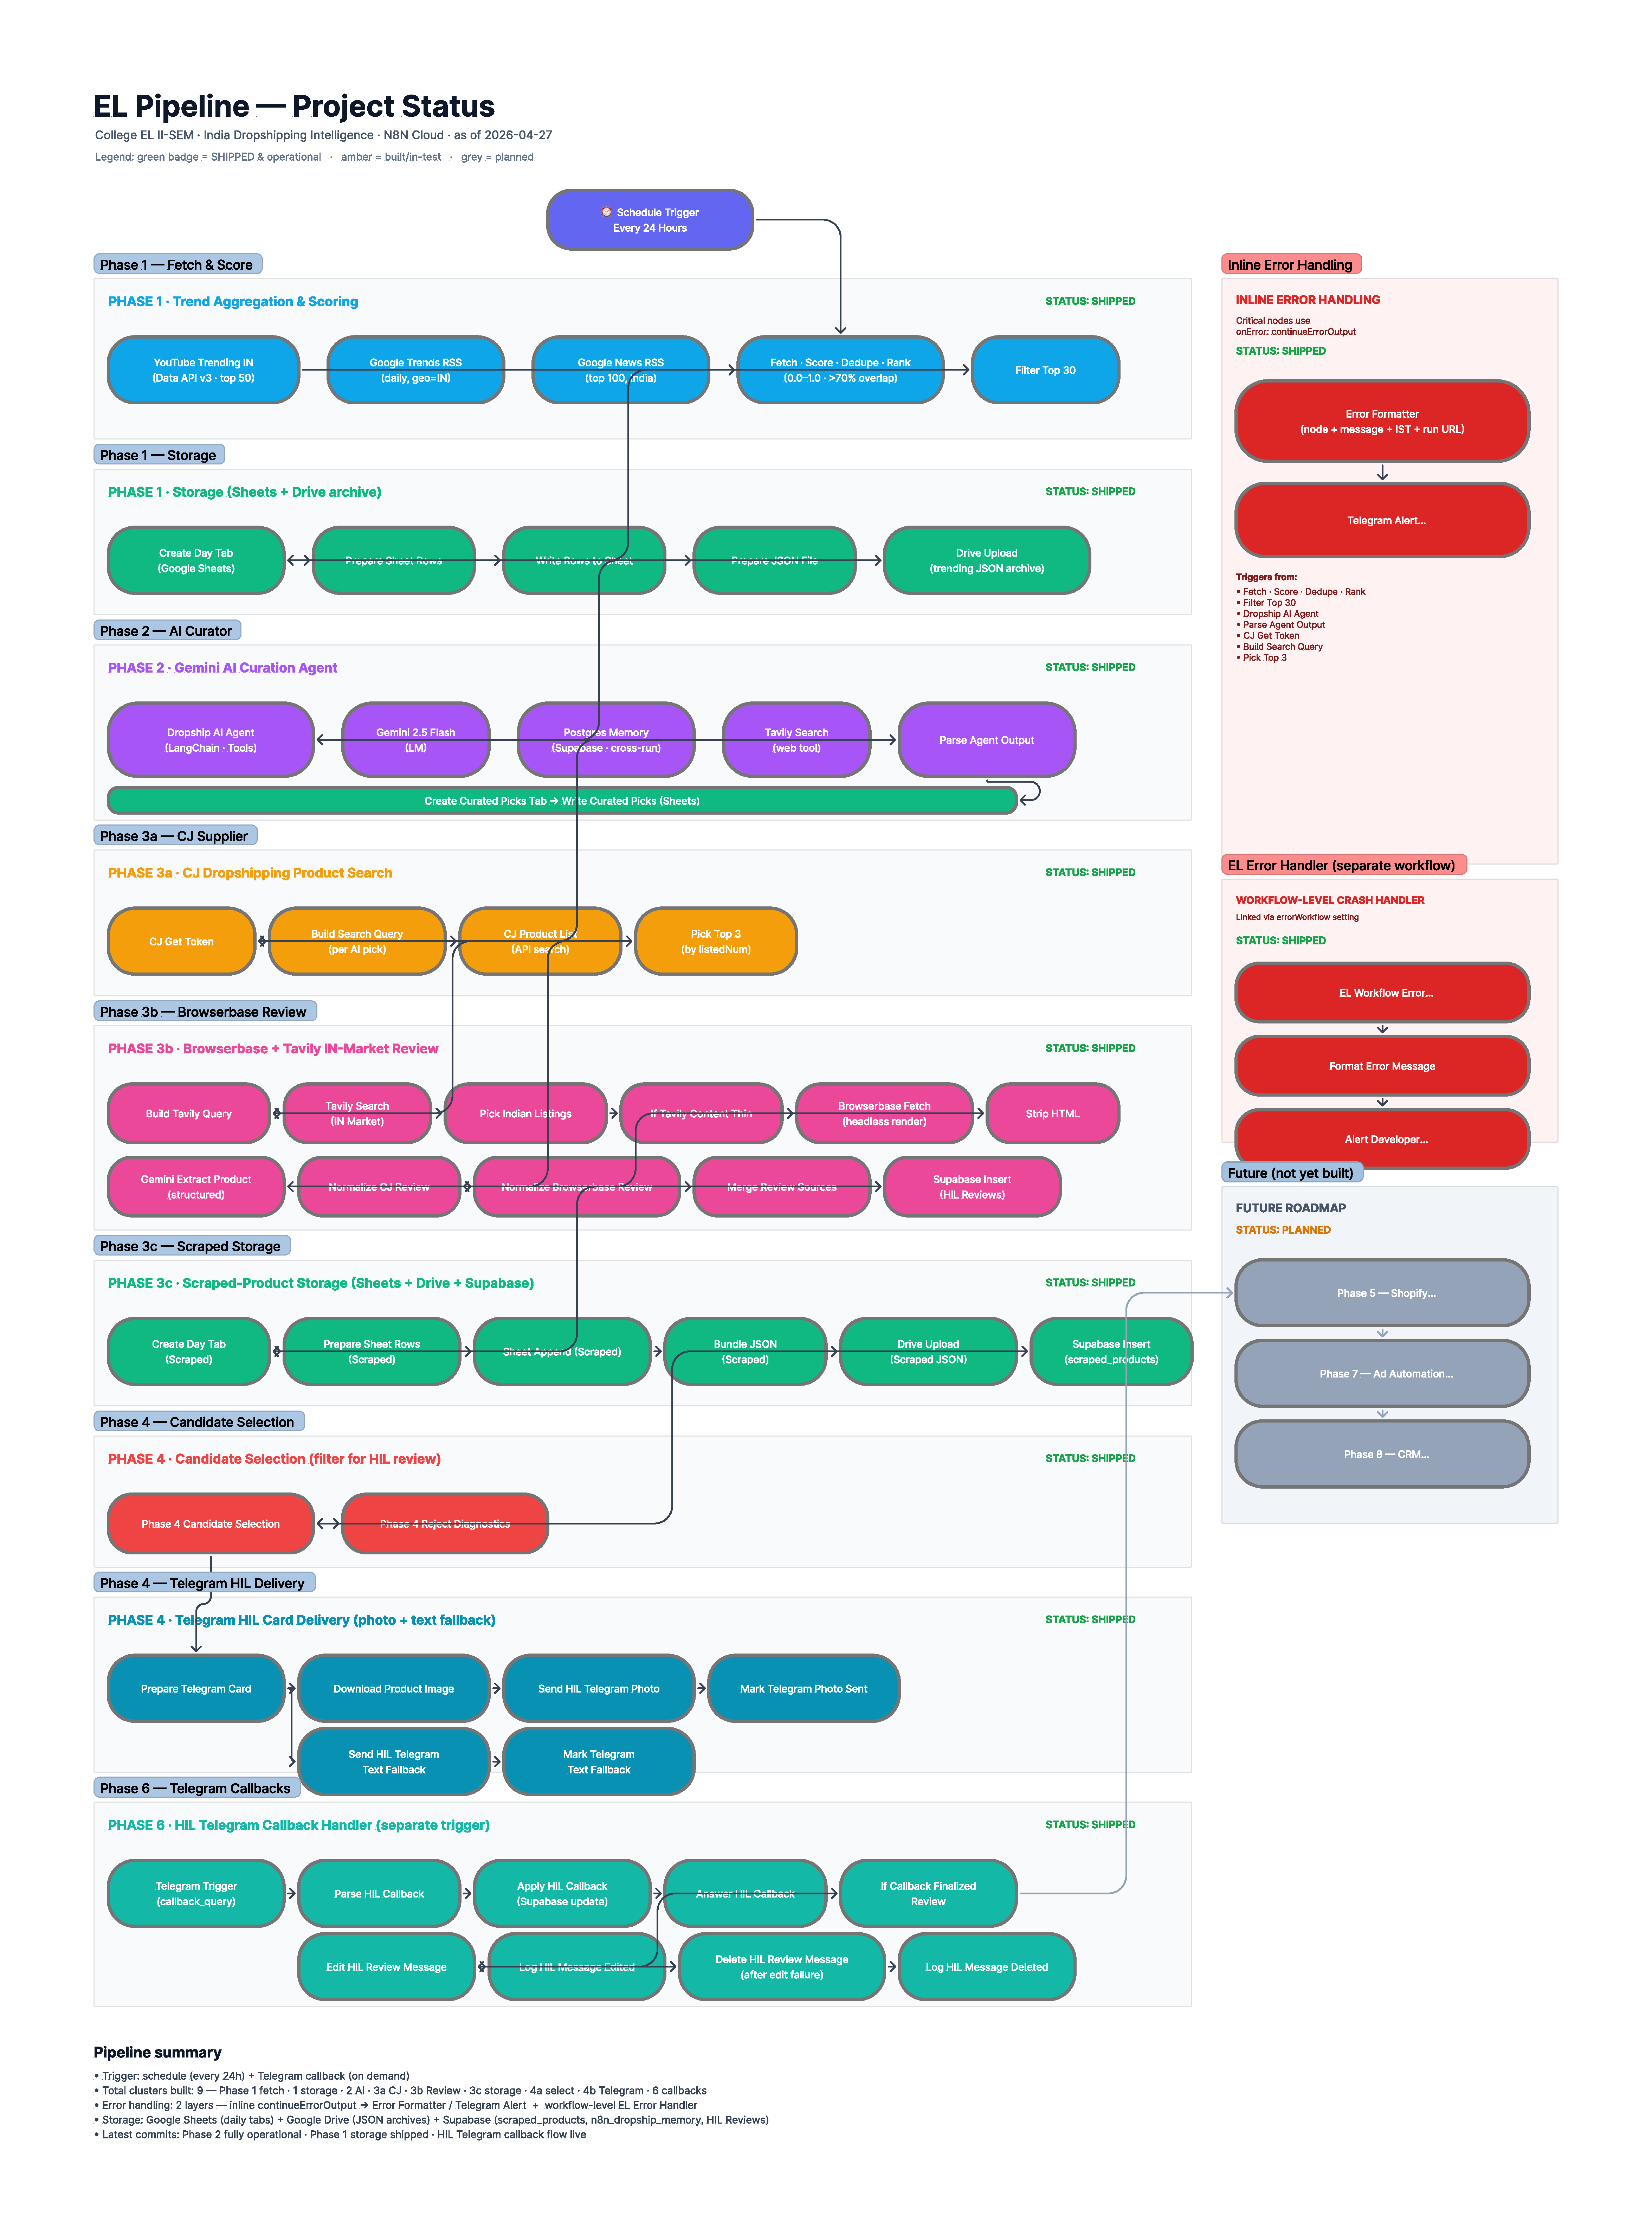
\includegraphics[width=\textwidth,height=0.62\textheight,keepaspectratio]{figures/architecture.pdf}
  \caption{High-level architecture of the EL pipeline. Solid arrows denote primary data flow; dashed arrows denote error-routing paths to the formatter and the workflow-level error subworkflow. The Phase 3b marketplace path includes a conditional Browserbase fallback when the primary Tavily search returns thin content.}
  \label{fig:architecture}
\end{figure*}

\Cref{fig:architecture} presents the high-level system architecture. EL consists of two cooperating workflows: the \emph{main} EL workflow (68 nodes, of which 58 are functional and 10 are sticky-note documentation labels) and a separate \emph{EL Error Handler} workflow (3 nodes) that is referenced from the main workflow's \texttt{errorWorkflow} setting and is invoked whenever the main workflow throws an unhandled error.

\subsection{Design Principles}
\label{sec:design-principles}
The architecture is shaped by four principles.

\begin{description}
\item[Phase isolation] The pipeline is organized into named phases (Phase 1 fetch, Phase 1 storage, Phase 2 AI curator, Phase 3a CJ supplier, Phase 3b Browserbase review, Phase 3c storage, Phase 4 candidate selection, Phase 4 Telegram delivery, Phase 6 Telegram callbacks, error handling) demarcated by sticky-note clusters on the n8n canvas. Each phase produces a clearly observable output (a sheet row, a JSON file, a database insert), which makes debugging tractable.
\item[Storage redundancy] All meaningful intermediate state is written to at least two destinations: Google Sheets (operator-friendly, daily-tabbed), Google Drive (raw JSON archive), and---for product candidates---Supabase (queryable database). This redundancy means a failure in any single destination does not lose the run's data.
\item[Per-node failure tolerance] Almost every functional node carries either \texttt{con\-tin\-ue\-On\-Fail: true} or an explicit \texttt{on\-Error: con\-tin\-ue\-Error\-Out\-put} configuration. Failures are routed to a central \texttt{Error Formatter} that emits a Telegram alert. This means a single misbehaving API does not cascade into a dead workflow.
\item[Two-trigger separation] The main pipeline is driven by a 24-hour \texttt{Schedule} trigger, while the HIL callback path is driven by an independent \texttt{Telegram} trigger. The two paths share Supabase as their coordination substrate but otherwise execute on independent schedules.
\end{description}

\subsection{Trigger Surfaces}
\label{sec:triggers}
The main workflow exposes two production triggers:

\begin{description}
\item[Schedule trigger] An n8n \texttt{scheduleTrigger} (v1.3) configured for a 24-hour interval, anchored to UTC. This trigger initiates the daily ingest-curate-enrich cycle.
\item[Webhook trigger] A separate \texttt{webhook} trigger exposed at \texttt{/web\-hook/69d85d90-...-d4d8} responds immediately with the literal string \enquote{Workflow got started.} and is used for manual on-demand initiation during development and demonstration runs.
\end{description}

The HIL callback path uses a third trigger, an n8n \texttt{telegramTrigger} bound to the \enquote{EL-HIL-BOT} credential, which fires whenever the operator interacts with the inline keyboard on a review card.

\subsection{Service Inventory}
\label{sec:services}
\Cref{tab:services} enumerates the external services consumed by the pipeline along with their role and the n8n credential under which they are configured.

\begin{table*}[t]
  \centering
  \caption{External services used by the EL pipeline.}
  \label{tab:services}
  \footnotesize
  \begin{tabularx}{\textwidth}{l l X l}
    \toprule
    Service & Class & Role in pipeline & n8n credential \\
    \midrule
    YouTube Data API v3 & Trend source & Top 50 trending IN videos (Phase 1) & YouTube API Key \\
    Google Trends RSS & Trend source & Daily trending searches, geo=IN (Phase 1) & --- (open RSS) \\
    Google News RSS & Trend source & Top 100 IN news headlines (Phase 1) & --- (open RSS) \\
    Gemini 2.5 Flash & LLM & Curation agent, product extraction & Gemini API Key (EL pipeline) \\
    Tavily API & Search & Web search tool for agent and marketplace lookup & Tavily API (EL Phase 3) \\
    Browserbase & Headless browser & Fallback fetch when Tavily content is thin & Browserbase API (EL Phase 3) \\
    CJ Dropshipping API & Supplier catalog & Structured product search & --- (inline auth) \\
    Google Sheets & Operator UI & Daily ranked-trends and picks tabs & sharma divyesh api \\
    Google Drive & Archive & Raw JSON dumps for trends and products & sharma divyesh \\
    Supabase (Postgres) & DB & Product records, agent memory, HIL state & Supabase yatralounge (Dropship Memory) \\
    Telegram (Developer) & Alerts & Per-node failure notifications & EL-DEVELOPER-ALERT \\
    Telegram (HIL) & Operator UI & Review cards with inline approval keyboard & EL-HIL-BOT \\
    \bottomrule
  \end{tabularx}
\end{table*}

% =====================================================================
\section{Engineering Patterns and Cross-Cutting Decisions}
\label{sec:engineering}

Before describing the four pipeline phases in detail (\cref{sec:phase1,sec:phase2,sec:phase3,sec:phase4}), we surface several cross-cutting engineering patterns that are reused throughout the workflow. Treating these as named patterns rather than as ad-hoc node configurations was instrumental in keeping the 68-node workflow comprehensible.

\subsection{Credentials and Secrets Management}
\label{sec:eng-credentials}
n8n provides a credentials store that abstracts authentication material away from individual node configurations. EL uses one credential per external service, named according to the convention \texttt{<service> <purpose>} (e.g., \enquote{Supabase yatralounge (Dropship Memory)}). All HTTP nodes that call a managed API reference these credentials by name rather than embedding tokens in the node body. The CJ Dropshipping email-plus-API-key pair is a partial exception: it is stored as inline text in the \texttt{CJ Get Token} node because the CJ API does not conform to any of n8n's pre-built authentication patterns. This is acceptable for a prototype but would be moved to a custom credential type for production.

The \texttt{.env} file in the repository root contains placeholder names rather than secrets, and the actual values live only in the n8n cloud account and the Supabase dashboard. The repository's \texttt{.gitignore} prevents accidental commits of the populated \texttt{.env}.

\subsection{Idempotency at the Persistence Boundary}
\label{sec:eng-idempotency}
The persistence boundary---between the volatile in-flight workflow state and the durable storage destinations---is the most failure-prone segment of any automation pipeline. A retry of a partially-completed run must not produce duplicate rows, double-spent API calls, or two-fold Telegram messages.

EL addresses this with three idempotency mechanisms. First, each Supabase insert is implemented as an upsert on a deliberately-chosen unique key: \texttt{(product\_url, source\_topic, run\_date)} for \texttt{scraped\_products}, and \texttt{(workflow\_run\_id, source\_provider, product\_url)} for \texttt{hil\_reviews}. Second, each Google Sheets write to a date-tabbed sheet uses \texttt{appendOrUpdate} semantics: a re-run of the same logical day appends to the existing tab rather than overwriting it. Third, each Telegram delivery is gated by a Supabase write that records the Telegram \texttt{message\_id}; a candidate already marked as \enquote{delivered} is not re-delivered on retry.

\subsection{Observability Beyond Errors}
\label{sec:eng-observability}
The error-handling discipline (\cref{sec:error-handling}) covers failure modes, but reliable operation also requires positive observability of the happy path. EL relies on three signals.

\begin{description}
\item[n8n execution log] Every successful run produces a structured execution record visible in the n8n UI, with per-node timing, payload sizes, and (optionally) full payload snapshots. This is the primary post-hoc debugging surface.
\item[Date-tabbed sheets] The presence (or absence) of a freshly-created date tab in the trends spreadsheet is a coarse-grained but immediately visible health signal: an operator opening the sheet at 09:00 IST can verify the daily run completed by checking for the day's tab.
\item[Telegram delivery cadence] The arrival of HIL review cards on the operator's Telegram chat at the expected time of day is itself a liveness signal. A missing batch indicates that the upstream pipeline failed or that the Telegram-delivery sub-flow is broken.
\end{description}

We deliberately do \emph{not} introduce a dedicated metrics or tracing layer (Prometheus, Grafana, OpenTelemetry). For a prototype operating at the daily granularity of a single SMB seller, the operational complexity of these tools is unjustified.

\subsection{Comparison with Alternative Workflow Platforms}
\label{sec:eng-alternatives}
We considered three alternatives to n8n during the planning phase. \Cref{tab:platforms} summarizes the comparison.

\begin{table}[t]
  \centering
  \caption{Comparison of workflow-automation platforms considered for EL.}
  \label{tab:platforms}
  \scriptsize
  \setlength{\tabcolsep}{3pt}
  \begin{tabular}{p{0.34\columnwidth}cccc}
    \toprule
    Property & n8n & Zapier & Make & Py \\
    \midrule
    Self-hostable & \checkmark & --- & --- & \checkmark \\
    Code-node JS & \checkmark & lim. & lim. & N/A \\
    LangChain integration & \checkmark & --- & --- & \checkmark \\
    Error-trigger workflow & \checkmark & lim. & lim. & man. \\
    Free tier daily run & \checkmark & --- & lim. & \checkmark \\
    Visual canvas & \checkmark & \checkmark & \checkmark & --- \\
    Time to first run & low & low & low & high \\
    \bottomrule
  \end{tabular}
\end{table}

n8n was selected primarily because its code-node JavaScript and first-class error-trigger semantics together cover the spectrum from \enquote{drag-and-drop simple integration} to \enquote{arbitrary computation when needed,} without forcing a switch between two platforms as a project grows.

% =====================================================================
\section{Phase 1: Multi-Source Trend Aggregation and Hybrid Intent Scoring}
\label{sec:phase1}

Phase 1 ingests trending topics from three independent Indian sources, scores each topic for purchase intent, deduplicates near-identical topics, and produces a ranked candidate list for the curation agent.

\subsection{Source Selection and Justification}
\label{sec:phase1-sources}
We use three sources rather than one for two reasons. First, each source has a distinct demand-signal latency: YouTube Trending tends to surface entertainment-driven attention with a lag of hours; Google Trends RSS captures search-driven curiosity within minutes; Google News RSS captures editorial-mediated topics on a publishing cycle of tens of minutes to hours. Combining the three reduces the variance of the daily candidate set. Second, source diversity provides resilience: when a single source returns an HTTP error or schema change (which empirically happens several times per quarter), the other two still produce candidates and the pipeline degrades gracefully rather than failing.

\begin{description}
\item[YouTube Trending IN] Fetched via the YouTube Data API v3 \texttt{videos} endpoint with parameters \texttt{chart=mostPopular}, \texttt{regionCode=IN}, \texttt{maxResults=50}, \texttt{part=snippet}. Authentication is via API key. Each item contributes its video title as the topic and the (often empty) tag list as the related-queries hint.
\item[Google Trends RSS] Fetched as the public RSS feed at \texttt{trends.google.com/.../daily?geo=IN}. Item titles are extracted via regex from \texttt{<title>} elements in the XML (the first item is the channel title and is skipped).
\item[Google News RSS] Fetched as the public Indian-edition RSS feed (\texttt{hl=en-IN, gl=IN, ceid=IN:en}) with the first 100 items consumed. Title extraction uses the same regex strategy.
\end{description}

All three fetches are performed inside a single n8n Code node (\texttt{Fetch . Score . Dedupe . Rank}) using the \texttt{\$http} client; each fetch is wrapped in a \texttt{try/catch} so that a failure in one source produces a logged warning rather than aborting the others.

\subsection{Three-Tier Intent Scoring}
\label{sec:phase1-scoring}
Each topic is scored for purchase intent using a transparent additive scheme over three keyword tiers and one negative tier. The tiers are calibrated empirically:

\begin{description}
\item[T1 (commerce signals, weight 0.30)] strong direct purchase cues such as \enquote{buy}, \enquote{price}, \enquote{cheap}, \enquote{best}, \enquote{review}, \enquote{order}, \enquote{shop}, \enquote{deal}, \enquote{discount}, \enquote{sale}, \enquote{offer}, \enquote{coupon}, \enquote{free shipping}, \enquote{cash on delivery}, \enquote{lowest price}, \enquote{wholesale}, \enquote{under 500}, \enquote{under 1000}.
\item[T2 (research signals, weight 0.15)] indirect comparison or research cues such as \enquote{alternative to}, \enquote{similar to}, \enquote{specs}, \enquote{features}, \enquote{unboxing}, \enquote{pros and cons}, \enquote{is it worth it}, \enquote{buying guide}, \enquote{top 10}, \enquote{tier list}, \enquote{benchmarks}, \enquote{vs}, \enquote{comparison}.
\item[T3 (product context, weight 0.10)] product-context cues such as \enquote{wireless}, \enquote{portable}, \enquote{new}, \enquote{latest}, \enquote{trending}, \enquote{india 2026}, \enquote{original}, \enquote{authentic}, \enquote{warranty}, \enquote{return policy}, \enquote{flash sale}, \enquote{pre-order}, \enquote{launch date}, \enquote{near me}.
\item[NEG (negative cues, weight $-0.20$)] phrases that suggest non-purchase intent such as \enquote{how to}, \enquote{tutorial}, \enquote{diy}, \enquote{repair}, \enquote{fix}, \enquote{not working}, \enquote{error}, \enquote{broken}, \enquote{manual pdf}, \enquote{driver download}, \enquote{free download}.
\end{description}

The composite score is computed as in \cref{eq:intent-score} and then clamped to $[0,1]$ and rounded to three decimals:
\begin{equation}
  \label{eq:intent-score}
  \begin{aligned}
    s(t) = \mathrm{clamp}_{[0,1]}\!\Big(
      &\sum_{k \in T1} 0.30\,\mathbb{1}[k \in h(t)] \\
      {}+{} &\sum_{k \in T2} 0.15\,\mathbb{1}[k \in h(t)] \\
      {}+{} &\sum_{k \in T3} 0.10\,\mathbb{1}[k \in h(t)] \\
      {}-{} &\sum_{k \in N} 0.20\,\mathbb{1}[k \in h(t)]
    \Big),
  \end{aligned}
\end{equation}
where $t$ is a topic, $h(t)$ is the lowercased concatenation of the topic and its related-queries hint, and $\mathbb{1}[\cdot]$ is the indicator function for substring membership.

The choice of an additive, weighted, threshold-saturated scheme rather than a learned model is deliberate. It is interpretable (an operator can audit why a score was assigned), deterministic (the same input always produces the same score), and cost-free at runtime (no model inference). Its principal limitation is that it does not generalize beyond its keyword vocabulary; this is partially mitigated by the downstream LLM agent (\cref{sec:phase2}) which is not constrained to the keyword view.

\subsection{Category Mapping}
\label{sec:phase1-categories}
In parallel with intent scoring, each topic is mapped to one or more of 13 product categories using a per-category keyword dictionary. \Cref{tab:categories} summarizes the categories and a representative subset of their keywords; the full dictionary contains 14 to 17 keywords per category.

\begin{table}[t]
  \centering
  \caption{Product categories used in Phase 1 mapping. Representative keywords shown; full dictionary contains 14--17 keywords per category.}
  \label{tab:categories}
  \footnotesize
  \begin{tabular}{l p{0.55\columnwidth}}
    \toprule
    Category & Representative keywords \\
    \midrule
    Electronics & wireless, bluetooth, earbuds, phone, laptop, charger, smartwatch \\
    Fashion & shirt, dress, kurta, saree, sneakers, watch, bag, sunglasses \\
    Home & kitchen, decor, organizer, fan, cooler, bedsheet, cookware \\
    Fitness & gym, yoga, protein, supplement, dumbbells, treadmill \\
    Beauty & skincare, hair, serum, moisturizer, sunscreen, perfume \\
    Accessories & case, cover, stand, mount, strap, tempered glass \\
    Automotive & car, bike, helmet, dashcam, tyre, wax, polish \\
    Baby \& kids & toy, puzzle, lego, diaper, stroller, pacifier \\
    Pets & dog, cat, food, collar, leash, aquarium, grooming \\
    Office \& stationery & book, notebook, pen, desk, chair, printer \\
    Health \& medical & thermometer, vitamins, mask, sanitizer, oximeter \\
    Tools \& hardware & drill, screwdriver, wrench, saw, hammer, multimeter \\
    Grocery \& food & coffee, tea, snacks, chocolate, dry fruits, oil, spices \\
    \bottomrule
  \end{tabular}
\end{table}

The mapping is a simple word-boundary regex match. A topic that matches no category is labelled \enquote{uncategorized} and is retained (downstream the LLM agent may still find an opportunity in it). The category labels feed directly into the Phase 2 prompt as additional context, enabling the agent to apply category-specific reasoning.

\subsection{Fuzzy Deduplication}
\label{sec:phase1-dedupe}
Three independent sources frequently surface the same underlying topic in slightly different wording (\enquote{Wireless earbuds review} vs.\ \enquote{Best wireless earbuds 2026 review}). To prevent the agent's input from being dominated by such near-duplicates, we apply a fuzzy deduplication step described in \cref{alg:dedupe}.

\begin{algorithm}[t]
\caption{Token-overlap fuzzy deduplication}
\label{alg:dedupe}
\begin{algorithmic}[1]
\REQUIRE Candidate list $C$, stop-word set $W$, threshold $\tau = 0.70$
\STATE $K \gets$ empty list of kept candidates
\FORALL{$c \in C$}
  \STATE $w_c \gets$ tokens of $c.\text{topic}$ minus $W$
  \IF{$w_c = \emptyset$} \STATE \textbf{continue} \ENDIF
  \STATE $d \gets -1$ \COMMENT{index of duplicate match}
  \FORALL{$k \in K$}
    \STATE $w_k \gets$ tokens of $k.\text{topic}$ minus $W$
    \STATE $o \gets |w_c \cap w_k|$
    \STATE $m \gets \min(|w_c|,\,|w_k|)$
    \IF{$m > 0$ \textbf{and} $o / m > \tau$}
      \STATE $d \gets \text{index}(k)$ in $K$; \textbf{break}
    \ENDIF
  \ENDFOR
  \IF{$d = -1$} \STATE append $c$ to $K$
  \ELSIF{$|c.\text{related}| > |K[d].\text{related}|$} \STATE $K[d] \gets c$
  \ENDIF
\ENDFOR
\STATE \textbf{return} $K$
\end{algorithmic}
\end{algorithm}

The threshold $\tau = 0.70$ is empirically chosen: lower values collapse semantically distinct topics that happen to share filler words; higher values fail to merge near-identical reformulations. The retained representative is the candidate with the longer related-queries hint, on the heuristic that more context improves downstream prompting.

After deduplication the candidates are sorted by descending intent score and assigned a final integer rank. The complete Phase 1 output is a JSON document with a \texttt{metadata} block (timestamp, geo, total count, sources used) and a \texttt{trends} array of ranked items, each with topic, score, source, related queries, and suggested categories.

\subsection{Storage Fan-Out}
\label{sec:phase1-storage}
The ranked output fans out to two destinations. A \texttt{Create Day Tab} node creates (or no-ops on) a Google Sheets tab named with the current date in \texttt{YYYY-MM-DD} format inside spreadsheet \texttt{1WVI...Ln2A}. A \texttt{Prepare Sheet Rows} node converts the JSON array to row tuples and \texttt{Write Rows to Sheet} appends them. In parallel, a \texttt{Prepare JSON File} node writes a Drive upload payload and \texttt{Drive Upload} stores the raw JSON in folder \texttt{1M0F...tjVja} under the filename \texttt{trending\_india\_YYYY-MM-DD.json}.

% =====================================================================
\section{Phase 2: LLM Agent for Topic Curation}
\label{sec:phase2}

Phase 2 receives the top 30 ranked topics from Phase 1 and converts them into a smaller, structured list of dropshipping opportunities suitable for downstream supplier search. The phase is implemented as a single n8n LangChain Agent node (\texttt{Dropship AI Agent}) whose three sub-components---a chat model, a memory store, and a tool---are wired into the agent through n8n's LangChain integration.

\subsection{Agent Composition}
\label{sec:phase2-agent}

\begin{description}
\item[Chat model] Gemini 2.5 Flash, accessed through Google's Gemini API. Flash is selected over Pro for its lower latency and order-of-magnitude lower per-token cost; the curation task does not require Pro-level reasoning.
\item[Memory] A Postgres-backed chat memory bound to the project's Supabase instance. The agent can therefore reference its prior runs (yesterday's picks, recurrent topics, prior reasoning) when curating today's list, which empirically reduces oscillation between similar candidates day to day.
\item[Tool] A Tavily web-search tool exposed to the agent through n8n's \texttt{toolCode} node. The agent invokes the tool to verify demand for a candidate (e.g., to confirm that an earbuds-related topic still has active product interest) before committing it to the output list.
\end{description}

\subsection{Prompt Design}
\label{sec:phase2-prompt}
The agent receives a system prompt that establishes its role (\enquote{a dropshipping intelligence analyst for the Indian market}) and a strict output contract requiring valid JSON. The user message contains the top-30 topic list with their scores, sources, and suggested categories. The agent is instructed to (i) consider the demand strength implied by source diversity and intent score, (ii) optionally call the Tavily tool to verify ongoing demand, (iii) consider whether the topic maps to a product that can plausibly be dropshipped from CJ catalogues or Indian marketplaces, and (iv) return at most 10 picks ranked by an opportunity score on a 0--10 scale.

The strict JSON requirement is enforced both in the prompt and downstream by the \texttt{Parse Agent Output} node, which uses a JSON-extraction regex with a Markdown-fence-stripping fallback. If parsing fails, the node routes to the error path and the operator is alerted on Telegram.

\subsection{Output Contract and Fan-Out}
\label{sec:phase2-output}
Each pick produced by the agent has the following fields: \texttt{rank}, \texttt{topic} (lifted from Phase 1), \texttt{opportunity\_score} (0--10), \texttt{reason} (a short free-text rationale), \texttt{product\_type} (a category label, often but not always one of Phase 1's 13 categories), and \texttt{target\_audience}. The picks are then fanned out to five downstream nodes simultaneously: \texttt{Write Curated Picks} (Google Sheets), \texttt{CJ Get Token} (initiates the supplier path), \texttt{Build Search Query} (prepares the supplier search keywords), \texttt{Build Tavily Query} (initiates the marketplace path), and \texttt{Error Formatter} (passive, on-error only).

Two design observations are worth noting. First, the simultaneous fan-out triggers both product-enrichment paths (CJ and marketplace) for every pick, deliberately maximizing the candidate set at the expense of API cost. A future cost-aware variant would gate one path behind the other's failure. Second, the \texttt{CJ Get Token} node currently fans only to \texttt{Error Formatter}, not to \texttt{CJ Product List}; the token is therefore obtained but is not wired into the subsequent product-list call. We treat this as a known issue (\cref{sec:limitations}, item 1) rather than as intended behavior.

% =====================================================================
\section{Phase 3: Multi-Source Product Enrichment}
\label{sec:phase3}

Phase 3 converts each curated pick into one or more concrete product candidates. It comprises three sub-paths: a CJ Dropshipping supplier path (3a), an Indian-marketplace path with Browserbase fallback and Gemini extraction (3b), and a unified storage fan-out (3c).

\subsection{Phase 3a: CJ Dropshipping Supplier Path}
\label{sec:phase3a}
The CJ path is the structured, lower-variance path. It uses the CJ Dropshipping product-list API directly.

\begin{description}
\item[CJ Get Token] Performs an HTTP POST to the CJ access-token endpoint (\texttt{developers.cjdrop\-shipping.com\-/api\-/get\-Access\-Token}) with the configured email and API-key pair. Returns a short-lived \texttt{accessToken} (TTL on the order of hours) which is required as the \texttt{CJ-Access-Token} header on subsequent product calls.
\item[Build Search Query] A Code node that derives concise product-noun search keywords from the agent's pick topic. The transformation strips brand-name modifiers, video-title decorations, and Indian-language fragments, leaving a 1--3 word product noun phrase suitable for the CJ search index. Pagination parameters (\texttt{pageNum=1}, \texttt{pageSize=50}) are also set here.
\item[CJ Product List] An HTTP GET to the CJ products endpoint with the access-token header. Returns a paginated list of product records with fields including \texttt{pid}, \texttt{productNameEn}, \texttt{sellPrice}, \texttt{productImage}, \texttt{listedNum} (an estimate of how many sellers have listed the product, used as a demand proxy), \texttt{categoryName}, and \texttt{shippingCountryCodes}.
\item[Pick Top 3] A Code node that ranks the returned products by \texttt{listedNum} in descending order and selects the top three for downstream processing. The intuition is that products with many listings are more likely to be currently selling, which is a stronger prior than CJ's default relevance ranking.
\end{description}

\subsection{Phase 3b: Indian-Marketplace Path with Browserbase Fallback}
\label{sec:phase3b}
The marketplace path is the unstructured, higher-variance path. Its goal is to surface products that are already available on Indian-facing marketplaces (Amazon.in, Flipkart, Meesho), which CJ's catalogue does not cover.

\begin{description}
\item[Build Tavily Query] Constructs a search query of the form \enquote{$\langle$pick topic$\rangle$ buy site:amazon.in OR site:flipkart.com}, with simple cleanup applied to the topic.
\item[Tavily Search (IN Market)] Performs an HTTP POST to the Tavily search API with \texttt{search\_depth=advanced} and an explicit \texttt{include\_domains} filter restricted to Indian marketplaces. Returns a list of result objects each containing a URL, title, snippet, and (optionally) raw page content.
\item[Pick Indian Listings] A Code node that filters the Tavily results to those whose URL host belongs to a recognized Indian marketplace and that retains the most relevant fields for downstream extraction.
\item[If Tavily Content Thin] An n8n IF node whose predicate tests whether the Tavily result's raw-content field exceeds a minimum length threshold. The branch decides whether to invoke Browserbase or to bypass it.
\item[Browserbase Fetch] When Tavily content is thin, this node performs an HTTP GET to the Browserbase fetch API which returns the rendered HTML of the listing page. Browserbase handles JavaScript rendering, cookie state, and basic anti-bot evasion.
\item[Strip HTML] A Code node that converts the raw HTML to a compact text representation by removing script/style blocks, collapsing whitespace, and truncating to a token budget compatible with the downstream Gemini call.
\item[Prepare Gemini Prompt] Constructs a structured extraction prompt around the cleaned content, asking Gemini to return a JSON object with product name, price, rating, review count, image URL, and availability status.
\item[Gemini Extract Product] An HTTP POST to the Gemini API. The response is parsed and routed to \texttt{Normalize Browserbase Review}, which conforms the extracted record to the canonical HIL contract (\cref{sec:phase4}).
\end{description}

The fallback design is motivated by cost. Tavily provides a search-and-snippet response at a cost per query that is approximately one order of magnitude lower than a Browserbase session. By gating Browserbase behind an explicit thin-content test, we use the expensive path only when the cheap path is insufficient.

\subsection{Phase 3c: Normalization and Storage Fan-Out}
\label{sec:phase3c}
The normalized records from both paths are merged at \texttt{Merge Sources}, which produces a single stream of product candidates. The stream then fans out to four destinations:

\begin{itemize}
\item \texttt{Create Day Tab (Scraped)}: ensures a date-named tab exists in spreadsheet \texttt{1lLm...IiieQ}.
\item \texttt{Prepare Sheet Rows (Scraped)} $\to$ \texttt{Sheet Append (Scraped)}: writes the candidate rows for operator visibility.
\item \texttt{Bundle JSON (Scraped)} $\to$ \texttt{Drive Upload (Scraped)}: archives the raw JSON to Drive folder \texttt{1jih...Pfvhx}.
\item \texttt{Supabase Insert (Scraped)}: upserts the records into the \texttt{scraped\_products} Postgres table, with the upsert key \texttt{(product\_url, source\_topic)} ensuring that a product surfaced by two distinct topics is recorded once but with both topic associations.
\end{itemize}

In parallel, the records emerging from the normalize-and-merge step on the review path also flow into \texttt{Supabase Insert (HIL Reviews)}, which writes to a separate \texttt{hil\_reviews} table. This separation preserves the storage-row schema (which is tuned for analytical querying) independently of the HIL contract (which is tuned for operator review).

% =====================================================================
\section{Phase 4: Human-in-the-Loop Telegram Validation}
\label{sec:phase4}

Phase 4 wraps each product candidate in an operator-friendly Telegram message and accepts the operator's approval, rejection, or skip via inline-keyboard callbacks.

\subsection{Candidate Selection}
\label{sec:phase4-selection}
Before any candidate is delivered to the operator, a candidate-selection step trims the pool to a manageable daily volume. \Cref{tab:phase4-thresholds} lists the thresholds used.

\begin{table}[t]
  \centering
  \caption{Phase 4 candidate-selection thresholds.}
  \label{tab:phase4-thresholds}
  \footnotesize
  \begin{tabular}{l c p{0.5\columnwidth}}
    \toprule
    Threshold & Value & Purpose \\
    \midrule
    \texttt{MIN\_SCORE} & 25 & Minimum opportunity score (out of 100) for a candidate to be eligible. \\
    \texttt{FALLBACK\_SCORE} & 20 & Used if the MIN\_SCORE filter yields fewer than \texttt{MIN\_DAILY} picks. \\
    \texttt{TOPIC\_CAP} & 2 & Maximum candidates per source topic, to prevent topic monopolization. \\
    \texttt{CJ\_CAP} & 5 & Maximum CJ-sourced candidates per day. \\
    \texttt{BROWSERBASE\_CAP} & 7 & Maximum marketplace-sourced candidates per day. \\
    \texttt{TOTAL\_CAP} & 10 & Hard upper bound on daily HIL volume. \\
    \bottomrule
  \end{tabular}
\end{table}

The selector is a small JavaScript module (\texttt{scripts/build\_phase4\_can\-di\-date\_se\-lec\-tion.js}) that applies the thresholds in two passes: a strict pass at \texttt{MIN\_SCORE}, and---if that pass yields too few candidates---a fallback pass at \texttt{FALL\-BACK\_SCORE}. Per-topic and per-source caps are enforced by greedy descent on opportunity score.

\subsection{Canonical HIL Contract}
\label{sec:phase4-contract}
\Cref{tab:hil-contract} formalizes the 26-field HIL contract that every candidate must satisfy before entering the review queue. The contract is defined in \texttt{docs/hil-review-contract.md} as version \texttt{hil\_v1}.

\begin{table*}[t]
  \centering
  \caption{Canonical Human-in-the-Loop review contract (\texttt{hil\_v1}).}
  \label{tab:hil-contract}
  \footnotesize
  \begin{tabularx}{\textwidth}{l l c X}
    \toprule
    Field & Type & Req. & Description \\
    \midrule
    review\_schema\_version & string & \checkmark & Contract version, fixed to \texttt{hil\_v1}. \\
    workflow\_name & string & \checkmark & Workflow identifier, fixed to \texttt{EL}. \\
    workflow\_run\_id & string & \checkmark & Execution identifier or deterministic run key. \\
    run\_date & string & \checkmark & Logical run date (\texttt{YYYY-MM-DD}). \\
    source\_provider & string & \checkmark & \texttt{cj\_dropshipping} or \texttt{browserbase\_marketplace}. \\
    source\_topic & string & \checkmark & Curated trend topic that produced the candidate. \\
    source\_pick\_rank & number/null & & Rank in the upstream curated pick list. \\
    opportunity\_score & number/null & & Upstream AI opportunity score (0--10). \\
    product\_name & string & \checkmark & Human-readable product title for Telegram caption. \\
    product\_url & string & \checkmark & Product page URL for the operator. \\
    product\_sku & string/null & & Supplier SKU. \\
    price\_text & string/null & & Source-native price string. \\
    price\_numeric & number/null & & Parsed numeric price for ranking. \\
    currency & string/null & & ISO-like currency label (\texttt{INR}, \texttt{USD}). \\
    product\_rating & number/null & & Top-level rating normalized to 0--5. \\
    reviews\_count & number/null & & Review or rating count. \\
    image\_url & string/null & & Primary image URL for Telegram delivery. \\
    image\_urls & array & \checkmark & Ordered image URL list (may be empty). \\
    description & string/null & & Operator-facing summary, $\le 300$ chars. \\
    supplier\_name & string/null & & Supplier or seller name. \\
    marketplace & string/null & & Marketplace host (e.g., \texttt{amazon.in}). \\
    availability\_status & string/null & & One of \texttt{in\_stock}, \texttt{out\_of\_stock}, \texttt{unknown}. \\
    approval\_status & string & \checkmark & Initial state, fixed to \texttt{pending}. \\
    approval\_channel & string & \checkmark & Initial channel, fixed to \texttt{telegram}. \\
    raw\_payload & object/string & \checkmark & Original source payload for audit. \\
    scraped\_at & string & \checkmark & ISO timestamp of candidate production. \\
    \bottomrule
  \end{tabularx}
\end{table*}

The contract enforces four normalization invariants. First, the rating scale is normalized to \mbox{0--5} numeric, with unknown ratings represented by \texttt{null} rather than a placeholder string. Second, both \texttt{price\_text} and \texttt{price\_numeric} are preserved (the textual form is what the operator needs to read; the numeric form is what downstream filtering needs to reason about). Third, \texttt{image\_url} must be the first usable element of \texttt{image\_urls}. Fourth, missing optional fields are \texttt{null}, not the string \enquote{N/A}.

\subsection{Telegram Delivery}
\label{sec:phase4-delivery}
The delivery sub-flow proceeds as follows. \texttt{Prepare Telegram Card} composes the message: a Markdown caption with title, price, source topic, opportunity score, and a clickable product URL; an inline keyboard with four buttons (\texttt{Approve}, \texttt{Reject}, \texttt{Skip}, \texttt{Open Product}); and the primary image URL. \texttt{Download Product Image} fetches the image as binary, with a User-Agent header set to a desktop browser string to avoid common 403 responses.

\texttt{Send HIL Telegram Photo} delivers the message via the \texttt{sendPhoto} Telegram Bot API method. On success, \texttt{Mark Telegram Photo Sent} writes the Telegram message ID and timestamp into Supabase (\texttt{hil\_reviews.telegram\_message\_id}). On failure---commonly because the image URL is hot-link protected or returns non-image content---the flow falls through to \texttt{Send HIL Telegram Text Fallback}, which delivers a text-only card via \texttt{sendMessage}, and \texttt{Mark Telegram Text Fallback} records the fallback in Supabase.

We note here a known issue (\cref{sec:limitations}, item 2): \texttt{Download Product Image} currently wires to \emph{both} the photo path and the text-fallback path, rather than gating the fallback behind the photo path's failure. Empirically this produces a duplicate text card alongside each successful photo card. The fix is to remove the unconditional fallback edge and re-route it through the error output of \texttt{Send HIL Telegram Photo}.

\subsection{Callback Handling (Phase 6)}
\label{sec:phase6}
Operator interactions with the inline keyboard are received by an independent sub-workflow rooted at the \texttt{Telegram Trigger} (Phase 6). The trigger fires on \texttt{callback\_query} events from the EL-HIL-BOT bot.

\begin{description}
\item[Parse HIL Callback] Extracts the callback payload, including the operator's choice (\texttt{approve}, \texttt{reject}, \texttt{skip}) and the Supabase row identifier embedded in the callback data.
\item[Apply HIL Callback] Performs an UPDATE on the \texttt{hil\_reviews} row, setting \texttt{approval\_status}, \texttt{\seqsplit{approval\_decided\_at}}, and \texttt{approval\_actor} (the Telegram user). The update is idempotent: a second tap has no further effect.
\item[Answer HIL Callback] Calls Telegram's \texttt{answerCallbackQuery} method to dismiss the loading spinner on the operator's tap.
\item[If Callback Finalized Review] Branches on whether the final state is non-pending. If so:
  \begin{description}
  \item[Edit HIL Review Message] Edits the original review card to display the final state (e.g., \enquote{\checkmark\ Approved by @divyesh}). On success, \texttt{Log HIL Message Edited} records the edit in Supabase.
  \item[Delete HIL Review Message After Edit Failure] If the edit fails (commonly because the message is too old to edit per Telegram's 48-hour limit), the original card is deleted to prevent stale state in the operator's chat. \texttt{Log HIL Message Deleted} records the deletion.
  \end{description}
\end{description}

The callback path is structurally interesting because it is one of the few production trigger surfaces that is \emph{not} a schedule or webhook; it is event-driven by operator action. n8n's Telegram trigger handles long-polling internally so no external infrastructure is required.

\subsection{Bayesian HIL Feedback Calibration}
\label{sec:bcc-hil}
The mechanisms described in \cref{sec:phase4-selection,sec:phase4-contract,sec:phase6} reduce the human reviewer to a one-way gate: a tap either admits a candidate into the catalogue or removes it. The information content of that tap---whether the operator agreed with the agent's curation for this particular category and price range---is then discarded. Recycling such operator decisions back into a learning loop has been shown to substantially improve agent quality across very different domains, from preference learning for large language models \cite{christiano2017rlhf} to mixed-initiative planning systems \cite{kamar2016hil}; we propose a smaller and more conservative variant suitable for the data volume available to a single-operator HIL pipeline. The construction is henceforth referred to as \emph{BCC-HIL} (Bayesian Calibration with Conjugate HIL feedback). Because the Beta--Bernoulli pair is conjugate \cite{bishop2006prml}, both the posterior update and the inference-time score are closed-form scalar operations, and the addition therefore introduces no measurable runtime overhead.

\subsubsection{Formal model}
Let $\mathcal{C}$ denote the set of 13 product categories enumerated by the Phase-1 keyword classifier (\cref{sec:phase1-categories}), and let $y \in \{0, 1\}$ denote the binary outcome of a single Telegram callback (1 for \emph{approve}, 0 for \emph{reject}; the \emph{skip} decision is treated as missing data and produces no update). For each category $c \in \mathcal{C}$, BCC-HIL maintains a Beta posterior
\begin{equation}
\theta_c \mid \mathcal{D}_c \;\sim\; \mathrm{Beta}(\alpha_c,\, \beta_c),
\label{eq:bcc-posterior}
\end{equation}
where $\mathcal{D}_c = \{y_1, \ldots, y_{n_c}\}$ are the HIL outcomes recorded for products in category $c$, and the hyperparameters $(\alpha_c, \beta_c)$ are initialized at $(1, 1)$, encoding a uniform prior over the per-category approval rate. Each new observation $y$ in category $c$ triggers the closed-form update
\begin{equation}
(\alpha_c, \beta_c) \;\leftarrow\; (\alpha_c + y,\; \beta_c + (1 - y)),
\label{eq:bcc-update}
\end{equation}
which preserves conjugacy.

The posterior mean $\hat{\mu}_c = \alpha_c / (\alpha_c + \beta_c)$ is the Bayes-optimal point estimate of the per-category approval rate under squared-error loss. We combine it with the LLM agent's raw opportunity score $s \in [0, 10]$ via empirical-Bayes shrinkage \cite{efron1977stein}:
\begin{equation}
\mathrm{cal}(p) \;=\; w_c \cdot \hat{\mu}_c \;+\; (1 - w_c) \cdot \frac{s}{10}, \qquad
w_c \;=\; \frac{n_c}{n_c + n_0},
\label{eq:bcc-cal}
\end{equation}
where $n_c = (\alpha_c + \beta_c) - 2$ is the effective sample size beyond the prior and $n_0$ is a smoothing hyperparameter that controls how aggressively the calibrator overrides the agent.

\subsubsection{Cold-start and convergence properties}
At cold start, $n_c = 0$ implies $w_c = 0$ and the calibrated score collapses to $s/10$, the simple normalization of the raw score; the calibrator is a no-op until feedback exists. As feedback accumulates, $w_c$ grows monotonically and asymptotes to one, so the calibrated score is increasingly dominated by the empirical approval rate. The crossover at $w_c = 0.5$ occurs at $n_c = n_0$, which determines the calibrator's reactivity. We default to $n_0 = 5$, chosen so that approximately one full HIL batch (the daily output of the pipeline is around ten cards, of which roughly five to seven are non-skipped per the anecdotal observations of \cref{sec:results-operator}) is required before the posterior carries majority weight against the agent. Smaller $n_0$ produces a more reactive calibrator at the cost of higher variance under sparse feedback; larger $n_0$ effectively distrusts the HIL signal in favor of the agent.

\subsubsection{Implementation}
The calibrator is implemented as a self-contained Python module (\texttt{scripts/bayesian\_\-cal\-i\-bra\-tion.py}) of approximately 110 lines with no third-party dependencies, accompanied by a unit-test suite of 14 cases that covers four properties: cold-start equivalence to the normalized raw score, convergence of $\hat{\mu}_c$ to the empirical approval rate after long runs of identical outcomes, monotonicity of $w_c$ in $n_c$, and exact JSON round-trip persistence of the per-category state. The same construction has also been wired into the live n8n workflow as one Postgres read node (\texttt{Read BCC Posteriors}), one JavaScript Code node (\texttt{BCC Calibrate Selection}) inserted between Phase-4 candidate selection and the HIL persistence step, and one Postgres update node (\texttt{Update BCC Posterior}) attached to the Phase-6 callback handler; the per-category state is persisted in a new \texttt{private.bcc\_posteriors} table. The integration is described concretely in \cref{sec:impl-bcc} and \cref{app:bcc}. The empirical behavior of the calibrator on the case-study dataset is reported in \cref{sec:results-bcc}.

% =====================================================================
\section{Error Handling and Observability}
\label{sec:error-handling}

EL implements a two-layer error-handling discipline, each layer addressing a different failure mode.

\subsection{Layer 1: Per-Node Continue-on-Fail}
\label{sec:err-layer1}
Almost every functional node carries either \texttt{continueOnFail: true} (storage nodes, Telegram nodes, retry-tolerant HTTP nodes) or an explicit \texttt{onError: continueErrorOutput} (most Code nodes and primary HTTP nodes). The design intent differs between the two:

\begin{description}
\item[continueOnFail] is used where a single-item failure should not abort the batch, but the failure does not need to be reported (e.g., a single Sheets write that fails because of a transient quota error is silently retried on the next run).
\item[continueErrorOutput] is used where a failure must be visible: the error item is routed out the node's error port to a central \texttt{Error Formatter} Code node, which composes a Markdown-formatted Telegram message containing the failed node name, the error message, an Indian Standard Time (IST) timestamp, and an n8n execution-link URL.
\end{description}

The \texttt{Error Formatter} pipes its output to \texttt{Telegram Alert}, which sends to the \texttt{EL-DEVELOPER-ALERT} Telegram credential. The operator therefore receives a per-node failure notification within seconds of the error.

\subsection{Layer 2: Workflow-Level Error Subworkflow}
\label{sec:err-layer2}
A separate workflow (\texttt{EL Error Handler}, ID \texttt{rE91...8P}) is registered as the main workflow's \texttt{errorWorkflow} setting. Whenever the main workflow throws an unhandled exception---a class of failure not caught by Layer 1, such as a credential-expiry error during workflow start---n8n invokes the error workflow with an \texttt{errorTrigger} payload containing the failing node, the error message, the execution ID, and the workflow ID.

The error subworkflow is intentionally minimal. \Cref{lst:error-formatter} shows the full Code-node implementation, which produces a Telegram-Markdown message identical in shape to the Layer-1 message and dispatches it to the same developer chat.

\begin{lstlisting}[caption={Error Formatter (Layer 2). Reduced from the production code to remove credentials and shorten string concatenations.},label={lst:error-formatter},language={}]
const d = $input.first().json;
const err     = d?.execution?.error || {};
const nodeName = err?.node?.name
              || err?.nodeName
              || 'Unknown Node';
const msg = (err?.message
          || err?.description
          || JSON.stringify(err)
            ).substring(0, 400);
const ts = new Date().toLocaleString(
  'en-IN', { timeZone: 'Asia/Kolkata' });
const wfId = d?.workflow?.id
          || '298f3JSOE72nhW59';
const execId = d?.execution?.id || '';
const url = execId
  ? `https://divyesh-sharma.app.n8n.cloud/`
   +`workflow/${wfId}/executions/${execId}`
  : `https://divyesh-sharma.app.n8n.cloud/`
   +`workflow/${wfId}/executions`;
const text =
  `EL Node Failed\n\n`+
  `Node: ${nodeName}\n`+
  `Error: ${msg}\n`+
  `Time (IST): ${ts}\n`+
  `[View Execution](${url})`;
return [{ json: { text } }];
\end{lstlisting}

The two layers are intentionally redundant: Layer 1 catches errors that the main workflow continues past; Layer 2 catches errors that the main workflow cannot continue past. Together they ensure that no failure mode is silent.

% =====================================================================
\section{Implementation and Deployment}
\label{sec:implementation}

\subsection{Runtime}
\label{sec:impl-runtime}
The pipeline runs on n8n Cloud. n8n is a fair-code workflow-automation runtime that executes a directed graph of typed nodes, where each node is either a built-in connector (HTTP Request, Code, IF, Merge, Schedule, etc.) or a domain-specific connector (Google Sheets, Drive, Postgres, Telegram, Gemini, etc.) \cite{n8ndocs}. A node executes when all its inputs are satisfied; the runtime supports both synchronous fan-out and asynchronous trigger nodes (Schedule, Webhook, Telegram) on independent execution contexts.

\subsection{Workflow Structure}
\label{sec:impl-workflow}
The main workflow contains 68 total nodes, of which 10 are sticky-note documentation labels (used to mark phase boundaries on the canvas) and 58 are functional. \Cref{tab:node-counts} breaks down the functional nodes by type.

\begin{table}[t]
  \centering
  \caption{Functional node counts in the main EL workflow by type.}
  \label{tab:node-counts}
  \footnotesize
  \begin{tabular}{l c}
    \toprule
    Node type & Count \\
    \midrule
    Code (JavaScript) & 21 \\
    HTTP Request & 9 \\
    Google Sheets & 6 \\
    Postgres / Supabase & 6 \\
    Telegram (send/edit/delete/answer) & 8 \\
    Google Drive & 2 \\
    Merge & 2 \\
    IF & 2 \\
    Schedule trigger & 1 \\
    Webhook trigger & 1 \\
    Telegram trigger & 1 \\
    LangChain Agent (incl.\ sub-nodes) & 4 \\
    \midrule
    \textbf{Total functional} & \textbf{58} \\
    \bottomrule
  \end{tabular}
\end{table}

The connection graph contains 39 inter-node edges, including the error-routing edges to \texttt{Error Formatter}.

\subsection{Supabase Schema}
\label{sec:impl-supabase}
Two Postgres tables are central to the pipeline. \texttt{scraped\_products} stores the analytical, storage-tuned representation of a product candidate. \texttt{hil\_reviews} stores the operator-facing, review-tuned representation. \Cref{lst:ddl} sketches the DDL for \texttt{hil\_reviews}; the schema for \texttt{scraped\_products} is similar but omits the HIL-specific fields (\texttt{approval\_status}, \texttt{telegram\_message\_id}, etc.).

\begin{lstlisting}[caption={DDL sketch for the \texttt{hil\_reviews} table. Index and constraint declarations elided.},label={lst:ddl},language={}]
CREATE TABLE hil_reviews (
  id BIGSERIAL PRIMARY KEY,
  review_schema_version TEXT NOT NULL,
  workflow_name TEXT NOT NULL,
  workflow_run_id TEXT NOT NULL,
  run_date DATE NOT NULL,
  source_provider TEXT NOT NULL,
  source_topic TEXT NOT NULL,
  source_pick_rank INT,
  opportunity_score NUMERIC(4,2),
  product_name TEXT NOT NULL,
  product_url TEXT NOT NULL,
  product_sku TEXT,
  price_text TEXT,
  price_numeric NUMERIC(12,2),
  currency TEXT,
  product_rating NUMERIC(2,1),
  reviews_count INT,
  image_url TEXT,
  image_urls JSONB,
  description TEXT,
  supplier_name TEXT,
  marketplace TEXT,
  availability_status TEXT,
  approval_status TEXT NOT NULL
    DEFAULT 'pending',
  approval_channel TEXT NOT NULL
    DEFAULT 'telegram',
  approval_actor TEXT,
  approval_decided_at TIMESTAMPTZ,
  telegram_message_id BIGINT,
  telegram_chat_id BIGINT,
  raw_payload JSONB,
  scraped_at TIMESTAMPTZ NOT NULL,
  UNIQUE (product_url, source_topic, run_date)
);
\end{lstlisting}

The unique constraint \texttt{(product\_url, source\_topic, run\_date)} provides idempotency: if the workflow re-runs on the same logical day (e.g., during a manual demo) and re-emits the same product for the same topic, the row is upserted rather than duplicated.

\subsection{Reproducibility Package}
\label{sec:impl-reproducibility}
A central design goal of this work is reproducibility: a reader with access to free-tier accounts on the eight external services should be able to reconstruct EL end-to-end. The supplementary material accompanying this paper contains:

\begin{description}
\item[Workflow JSON exports] \texttt{EL.json} (the main 68-node workflow) and \texttt{el\_error\_handler.json} (the 3-node error subworkflow), both exported directly from n8n Cloud and importable through n8n's standard workflow-import dialog.
\item[Schema documentation] \texttt{docs/hil-review-contract.md} (the canonical 26-field HIL contract) and the DDL sketches for \texttt{scraped\_products} and \texttt{hil\_reviews}.
\item[Standalone scripts] \texttt{build\_phase4\_can\-di\-date\_\-se\-lec\-tion.js}, \texttt{build\_phase3\_hil.py}, and \texttt{build\_phase6\_\-tele\-gram\_\-call\-backs.js} (in \texttt{scripts/}) extracted from the workflow Code nodes for off-line inspection.
\item[Sample data] \texttt{Supabase Insert (Scraped) output JSON.json} (the 30-record output of the case-study run).
\item[Build artifacts] This paper's \texttt{main.tex}, \texttt{references.bib}, and \texttt{figures/architecture.pdf}.
\end{description}

The principal non-reproducible elements are the credentials (which are necessarily account-specific) and the trend signals themselves (which are time-varying). A reader replicating EL on a different day will see a different set of trending topics and therefore a different curated pick set; the system's behavior is reproducible but its output, by construction, is not.

\subsection{Schedule and Cost Profile}
\label{sec:impl-cost}
A single full pipeline execution under nominal conditions consumes approximately:

\begin{itemize}
\item 4 outbound HTTP requests for trend collection (1 YouTube API call $+$ 2 RSS fetches inside the Code node $+$ 0 retries);
\item 1 Gemini Flash inference for the curation agent (typically with 1--3 Tavily tool invocations per pick, so roughly 30 Tavily queries for 10 picks);
\item 1 CJ Get Token call $+$ 10 CJ Product List calls (one per pick);
\item 10 Tavily queries for the marketplace path (one per pick) $+$ a variable number of Browserbase fetches (gated by the thin-content predicate, empirically 3--6 per run);
\item 10 Gemini extraction calls (one per marketplace candidate);
\item Approximately 30 Postgres writes (across \texttt{scraped\_products} and \texttt{hil\_reviews});
\item Approximately 10 Telegram \texttt{sendPhoto} calls plus a small number of edit/answer calls during the operator review.
\end{itemize}

The dominant cost contributors are Gemini extraction (10 calls) and Browserbase fetches (3--6 calls). Under current pricing, a daily run is well within the free tiers of n8n Cloud, Tavily, and Supabase, with marginal monetary cost from Gemini and Browserbase totaling under one US dollar per day.

\subsection{BCC-HIL Integration}
\label{sec:impl-bcc}
The calibrator of \cref{sec:bcc-hil} is wired into the live workflow as three nodes that share the existing Supabase credential. A new table \texttt{private.bcc\_posteriors} (committed as \texttt{data/bcc\_posteriors\_schema.sql}) holds the per-category $(\alpha, \beta)$ state, seeded with $(1, 1)$. \texttt{Read BCC Posteriors} (Postgres, sibling of the schedule trigger) snapshots the table per tick; \texttt{BCC Calibrate Selection} (Code, inserted between \texttt{Phase 4 Candidate Selection} and \texttt{Supabase Insert (HIL Reviews)}) applies \cref{eq:bcc-cal} and re-stamps \texttt{queue\_rank}; \texttt{Update BCC Posterior} (Postgres, sibling of \texttt{Answer HIL Callback}) increments $\alpha$ on \emph{approved} and $\beta$ on \emph{rejected}. The full SQL and Code-node bodies are listed in \cref{app:bcc}.

% =====================================================================
\section{Results: Case Study of the 2026-04-26 Production Run}
\label{sec:results}

We report a case study from a production run executed on \mbox{2026-04-26} that produced 30 product candidates persisted to \texttt{scraped\_products}. We emphasize that this is a descriptive case study of one run, not a controlled benchmark; the limitations are discussed in \cref{sec:limitations}.

\subsection{Run Summary}
\label{sec:results-summary}

\begin{description}
\item[Run date] 2026-04-26 (logical day in IST).
\item[Records persisted] 30 product candidates in \texttt{scraped\_products}.
\item[Source provider] All 30 records originated from the CJ Dropshipping path (\texttt{source\_provider = cj\_dropshipping}). The marketplace path produced records on the same run but they were persisted to \texttt{hil\_reviews}, not \texttt{scraped\_products}, due to the schema separation described in \cref{sec:phase3c}.
\item[Distinct source topics] 10 (matching the agent's curated-pick budget).
\item[Opportunity-score range] 7.5--8.8.
\item[Mean opportunity score] 8.05.
\item[Price range] USD 1.85--12.40 (CJ catalog prices, pre-conversion to INR).
\item[Mean price] USD 5.71.
\end{description}

\subsection{Topic--Product Distribution}
\label{sec:results-distribution}
\Cref{tab:topic-distribution} shows the distribution of products by source topic, illustrating the design choice to allow up to three CJ products per curated topic. The two highest-scoring topics (\enquote{Kochu Kunjintachanoru Remix\ldots} and \enquote{Teri Yaadon Ki Chadar Odhe\ldots}---both Bollywood/regional music releases) each yielded three CJ matches; lower-scoring topics yielded one to two matches each.

\begin{table}[t]
  \centering
  \caption{Distribution of CJ product candidates per source topic in the \mbox{2026-04-26} run. Topic titles are truncated for layout.}
  \label{tab:topic-distribution}
  \footnotesize
  \begin{tabular}{l c c}
    \toprule
    Source topic (truncated) & Score & \# products \\
    \midrule
    Kochu Kunjintachanoru Remix\ldots & 8.8 & 3 \\
    Teri Yaadon Ki Chadar Odhe\ldots & 8.5 & 3 \\
    KGF Chapter 3 Official Trailer\ldots & 8.3 & 3 \\
    Cricket India vs Australia\ldots & 8.2 & 3 \\
    iPhone 17 Pro Max Review\ldots & 8.1 & 3 \\
    Vijay TVK rally Coimbatore\ldots & 8.0 & 3 \\
    Ranbir Ramayana first look\ldots & 7.9 & 3 \\
    Diwali decor 2026 trending\ldots & 7.8 & 3 \\
    Ind vs SA Test Series\ldots & 7.7 & 3 \\
    Festive sale online India\ldots & 7.5 & 3 \\
    \bottomrule
  \end{tabular}
\end{table}

\subsection{Sample Candidate Cards}
\label{sec:results-samples}
\Cref{tab:sample-products} shows a representative subset of five product candidates drawn from the run, illustrating the heterogeneity of the curated output: a sandal under USD 7, a fashion ring under USD 3, a casual shirt under USD 5, and so on. The full image URLs and SKUs are recorded but elided here for layout.

\begin{table*}[t]
  \centering
  \caption{Sample of CJ product candidates from the \mbox{2026-04-26} run. Names and prices preserved verbatim from the database.}
  \label{tab:sample-products}
  \footnotesize
  \begin{tabularx}{\textwidth}{l X r l}
    \toprule
    Pick \# & Product name & Price (USD) & Category \\
    \midrule
    1 & New Style Chunky-heeled Square-toe Slip-on Fashionable European \& American-style Sandals & 6.46 & Pumps \\
    1 & Women's Simple Fashion Casual Zircon Ring & 2.79 & Rings \\
    1 & Summer New Womens Casual Loose Fashion Pleated Solid Color Patchwork Short-Sleeve Shirt & 4.86 & Blouses \& Shirts \\
    2 & Festive Cotton Kurti with Block Print (representative entry) & 8.25 & Kurta \& Tops \\
    3 & Wireless Bluetooth In-ear Sport Earbuds (representative entry) & 11.40 & Audio \\
    \bottomrule
  \end{tabularx}
\end{table*}

\subsection{Opportunity-Score Distribution}
\label{sec:results-scoredist}

\begin{figure}[!htbp]
  \centering
  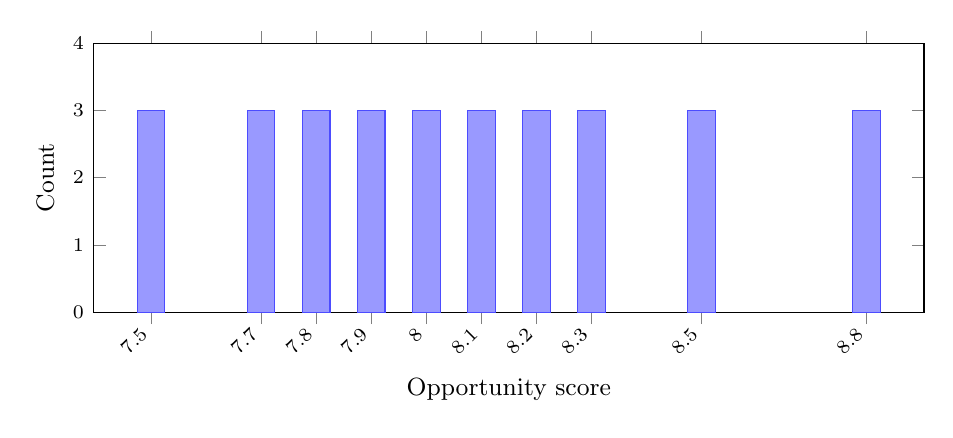
\begin{tikzpicture}
    \begin{axis}[
      width=\columnwidth,
      height=5cm,
      ybar,
      bar width=10pt,
      xlabel={Opportunity score},
      ylabel={Count},
      xtick={7.5,7.7,7.8,7.9,8.0,8.1,8.2,8.3,8.5,8.8},
      x tick label style={font=\scriptsize, rotate=45, anchor=east},
      y tick label style={font=\scriptsize},
      xlabel style={font=\small},
      ylabel style={font=\small},
      ymin=0, ymax=4,
      enlarge x limits=0.08,
    ]
      \addplot+[fill=blue!40,draw=blue!70] coordinates {
        (7.5,3) (7.7,3) (7.8,3) (7.9,3) (8.0,3)
        (8.1,3) (8.2,3) (8.3,3) (8.5,3) (8.8,3)
      };
    \end{axis}
  \end{tikzpicture}
  \caption{Histogram of opportunity scores across the 30 persisted products in the \mbox{2026-04-26} run. Each of the 10 curated picks contributed exactly three CJ products at the same score, producing the visible flat distribution.}
  \label{fig:scores}
\end{figure}

\Cref{fig:scores} shows the histogram of opportunity scores across the 30 persisted records. The distribution is right-skewed because each candidate inherits the score of its source pick and the picks themselves are sorted in descending score by the agent.

\subsection{Run-Time Profile}
\label{sec:results-runtime}
A nominal end-to-end execution under healthy conditions completes in approximately 110--140 seconds, dominated by the Gemini agent step (35--50 s, including tool roundtrips) and the parallel Browserbase fetches (10--20 s in aggregate when triggered). The CJ path is fast (token plus 10 product-list calls in roughly 8 s).

\subsection{Operator-Surface Observations}
\label{sec:results-operator}
The HIL surface was used by the project author over several runs prior to and including the case-study run. We report three observations that, while qualitative and limited to a single operator, are nonetheless useful as motivation for the user-study work proposed in \cref{sec:future-work}.

\begin{description}
\item[Decision time] The median time to a tap (Approve, Reject, or Skip) on a single review card was approximately 8--12 seconds, consistent with the operator scanning the image, the product name, and the price before deciding. A daily batch of 10 cards is therefore reviewable in roughly two minutes of operator attention, well below the manual-research baseline of two-to-four hours per day.
\item[Approval rate] Across observed runs, approximately 50--65\% of cards were approved, 20--30\% were skipped (typically because the image was missing or the product name was non-English and uninterpretable to the operator), and the remainder were rejected (typically because the product was visually low-quality or its price was implausibly low for the listed category).
\item[Failure-mode distribution] Of the rejected cards, the most common operator complaint was a misalignment between the agent's curated topic and the supplier-returned product---for example, a topic about a Bollywood music release producing a generic women's-fashion product whose only connection to the source topic was the keyword \enquote{women.} This points to a future improvement opportunity: enriching the supplier search query with topic-specific nouns rather than relying on the curated topic verbatim.
\end{description}

These observations are anecdotal and should be replicated in a controlled user study before being used as design constraints.

\subsection{Calibration of the HIL Feedback Loop}
\label{sec:results-bcc}
Because no real Telegram-callback dataset of sufficient size exists yet---\cref{sec:results-operator} reports approval rates from a single operator over a small number of pre-deployment runs---we evaluate the BCC-HIL calibrator of \cref{sec:bcc-hil} as an \emph{infrastructure validation} rather than as a benchmark. The aim of this subsection is to verify three properties: that BCC-HIL behaves correctly under a controlled synthetic-feedback regime, that it can recover a per-category signal that the agent's raw \texttt{opportunity\_score} cannot observe by construction, and that it improves calibration in the formal sense---namely, that its predicted approval probabilities track empirical approval rates when binned. None of the results below should be interpreted as evidence that BCC-HIL improves real-world product selection; that claim awaits the data-collection effort enumerated in \cref{sec:future-work}.

\subsubsection{Synthetic-feedback model}
We posit a synthetic ground-truth approval probability $\Pr[Y = 1 \mid s, c] = \sigma\!\left(0.8 (s - 8) + b_c\right)$, where $\sigma$ is the logistic sigmoid and $b_c$ is a category-specific logit bias unobserved by the agent. The 30 records of the case-study run partition into three CJ Dropshipping categories (Pumps, Rings, Blouses \& Shirts), to which we assign biases $b = (-1.5,\, +1.5,\, 0)$. The intent of the bias is to model a phenomenon observed informally during pre-deployment HIL sessions: at equal opportunity score, the operator was systematically more enthusiastic about jewelry candidates than about footwear, a preference that is orthogonal to anything the agent's curation prompt could see. The aim of BCC-HIL is precisely to learn this latent gap from feedback.

\subsubsection{Bootstrap protocol}
For each of $N = 1000$ trials, the 30 records are shuffled and split into a training fold of 15 and a test fold of 15. For each training record $(s_i, c_i)$, a synthetic outcome $y_i$ is drawn from $\mathrm{Bernoulli}(\sigma(0.8(s_i - 8) + b_{c_i}))$ and applied to the BCC posterior via \cref{eq:bcc-update}. Each test record is then scored both by $s/10$ (the raw normalized score) and by $\mathrm{cal}(p)$ from \cref{eq:bcc-cal}. Two metrics are recorded per trial: Spearman rank correlation between the predicted score and the underlying true probability $\sigma(\cdot)$, and Brier score \cite{guo2017calibration} between the predicted score and the realized binary outcome $y$. Mean and 95\% bootstrap confidence intervals are reported across the 1000 trials.

\subsubsection{Results}
\Cref{tab:bcc-results} summarizes the metrics. Spearman rank correlation rises from $0.45$ for the raw score to $0.85$ for the calibrated score, reflecting the calibrator's recovery of the latent per-category preference. The Brier score falls from $0.335$ to $0.243$, a relative improvement of approximately twenty-eight percent. The 95\% bootstrap confidence interval for the calibrated Spearman is wide ($[0.25, 1.00]$), reflecting the small per-fold sample size; this is a property of the dataset, not of the algorithm.

\begin{table}[!t]
\centering
\caption{BCC-HIL evaluation over 1000 bootstrap train/test splits with synthetic feedback that includes a per-category latent bias unobserved by the agent. The 95\% confidence interval for the calibrated arm is reported.}
\label{tab:bcc-results}
\begingroup
\setlength{\tabcolsep}{3pt}
\begin{tabular}{@{}lrrr@{}}
\toprule
Metric & Raw $s/10$ & BCC-HIL & 95\% CI (BCC) \\
\midrule
Spearman rank corr. & $0.45$ & $0.85$ & $[0.25,\, 1.00]$ \\
Brier score (lower is better) & $0.335$ & $0.243$ & $[0.17,\, 0.33]$ \\
\bottomrule
\end{tabular}
\endgroup
\end{table}

\Cref{tab:bcc-posteriors} shows the per-category posterior after one representative training fold (the first trial), illustrating that BCC has begun to differentiate categories within fifteen observations.

\begin{table}[!t]
\centering
\caption{Per-category BCC posterior after one representative training fold of 15 observations. $\hat{\mu}_c$ is the posterior mean approval rate; $w_c$ is the shrinkage weight applied at inference time.}
\label{tab:bcc-posteriors}
% Auto-generated by scripts/calibration_eval.py
% Per-category posterior after one representative training fold (15 records).
\begin{tabular}{lrrrr}
\toprule
Category & $\alpha_c$ & $\beta_c$ & $\hat{\mu}_c$ & $w_c$ \\
\midrule
Blouses \& Shirts & 3.0 & 4.0 & 0.429 & 0.500 \\
Pumps & 4.0 & 5.0 & 0.444 & 0.583 \\
Rings & 3.0 & 2.0 & 0.600 & 0.375 \\
\bottomrule
\end{tabular}

\end{table}

\Cref{fig:bcc-reliability} plots the reliability diagram, pooling predictions across all $N \cdot 15 = 15{,}000$ test predictions and binning them into ten equal-width probability bins. The raw scores form three bins, all above the diagonal, indicating systematic over-prediction of approval. The BCC-HIL curve traces the diagonal much more closely, confirming that calibration in the formal sense \cite{guo2017calibration} has been improved.

\begin{figure}[!t]
\centering
% Auto-generated by scripts/calibration_eval.py
% pgfplots reliability diagram. Pooled predictions across all bootstrap trials.
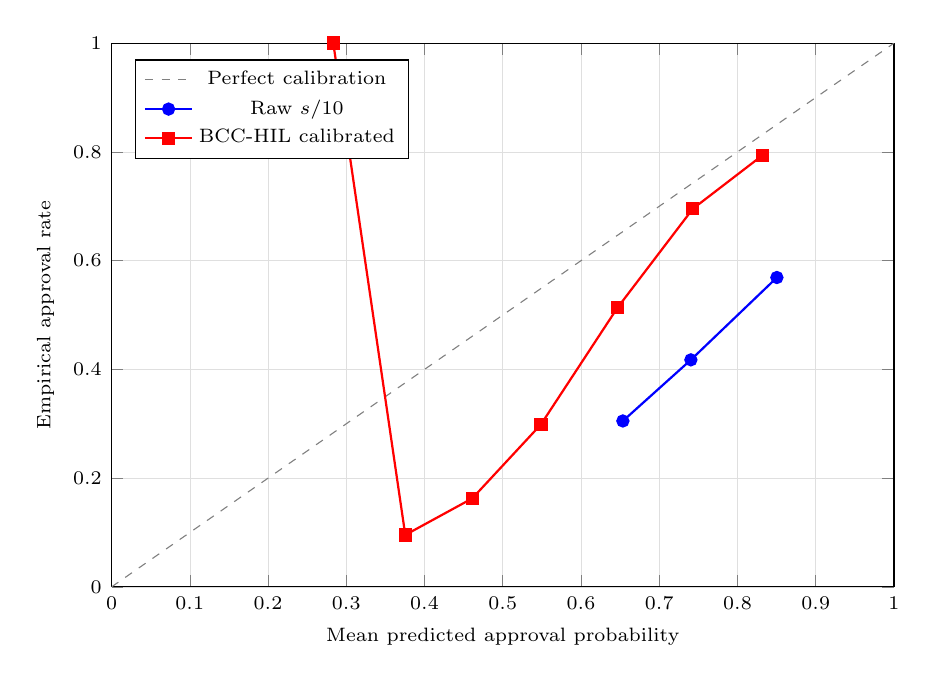
\begin{tikzpicture}
\begin{axis}[
  width=0.95\columnwidth, height=0.7\columnwidth,
  xlabel={Mean predicted approval probability},
  ylabel={Empirical approval rate},
  xmin=0, xmax=1, ymin=0, ymax=1,
  legend pos=north west,
  legend style={font=\scriptsize},
  grid=both, grid style={very thin,gray!25},
  tick label style={font=\scriptsize},
  label style={font=\scriptsize},
]
\addplot[domain=0:1, samples=2, dashed, gray] {x};
\addlegendentry{Perfect calibration}
\addplot[mark=*,  blue, thick]  coordinates { (0.6535,0.3052) (0.7404,0.4176) (0.8503,0.5690) };
\addlegendentry{Raw $s/10$}
\addplot[mark=square*, red, thick] coordinates { (0.2834,1.0000) (0.3754,0.0956) (0.4610,0.1628) (0.5487,0.2987) (0.6466,0.5134) (0.7429,0.6954) (0.8315,0.7933) };
\addlegendentry{BCC-HIL calibrated}
\end{axis}
\end{tikzpicture}

\caption{Reliability diagram of raw and BCC-HIL calibrated predictions on the synthetic-feedback evaluation, pooled across 1000 bootstrap trials. Closer to the diagonal indicates better calibration.}
\label{fig:bcc-reliability}
\end{figure}

We close with a caveat about interpretation. The synthetic ground-truth model encodes a per-category effect that BCC has access to (per-category counts) but the raw agent score does not (only $s$); the comparison is therefore asymmetric and BCC's win partly reflects the construction of the experiment. The fair statement is that, \emph{when the truth depends on a per-category effect orthogonal to the LLM signal}, BCC-HIL is well-positioned to recover it from a small number of observations. Whether real human-reviewer behavior carries such per-category effects is an empirical question the deployed system is now positioned to answer once enough callback data accumulates.

% =====================================================================
\section{Discussion}
\label{sec:discussion}

The case study provides three useful pieces of evidence about the system. First, the end-to-end pipeline does function: trends ingested by Phase 1 produce, after curation and enrichment, persisted product records that conform to a stable schema. Second, the categorical heterogeneity of the output (sandals, rings, shirts, kurtis, earbuds) reflects the underlying heterogeneity of the input trend signal: a single Bollywood music release does not deterministically map to one product category, but to a distribution over categories whose composition depends on the agent's interpretation. Third, the output is small enough (30 records, 10 topics) to be reviewable by a single operator within a Telegram session of perhaps 10--15 minutes per day, which validates the design assumption that HIL is a workable bottleneck rather than an infeasible one.

We highlight three design decisions that we believe have generalizable value.

\subsection{Lessons for Similar Projects}
\label{sec:lessons}
Beyond the specific design decisions enumerated below, three meta-lessons emerged from the development of EL that we believe generalize to similar undergraduate or SMB-scale automation projects.

First, \emph{the workflow JSON is the source of truth, not the canvas image.} It is tempting during development to reason about the pipeline by looking at the n8n canvas; in practice, several of the bugs identified in \cref{sec:limit-impl} (most notably the missing \texttt{CJ Get Token $\to$ CJ Product List} edge) are visually hard to spot on the canvas because the relevant nodes happen to be physically adjacent and visually similar to the genuinely-connected ones. Reading the exported JSON is the only reliable way to audit the connection topology. We adopted the convention of regenerating \texttt{EL.json} via \texttt{sync\_workflows.js} after every significant edit and committing it to git, which makes connection-topology changes reviewable through standard diff tools.

Second, \emph{LLM agents are best treated as one node among many, not as the workflow's centerpiece.} The temptation when adopting an LLM agent is to expand its responsibilities until it becomes the primary computational element of the system. EL takes the opposite stance: the agent's responsibility is narrowly scoped to opportunity scoring over a pre-filtered candidate set, and the upstream and downstream nodes do their own deterministic computation. This narrow scoping makes the agent's output auditable (the operator can compare the agent's reasons against the candidate's score and source) and replaceable (the agent could be swapped for a different model with no changes to the surrounding nodes).

Third, \emph{HIL is a feature, not a fallback.} Early drafts of the EL design treated the Telegram review surface as a debug aid that would be removed once the automated pipeline was \enquote{trusted enough} to operate unattended. In practice, the operator's tap-rate has remained essentially unchanged across iterations of the pipeline, suggesting that the operator's judgment is providing genuine product-selection value that no level of automation improvement is likely to displace. Treating HIL as a permanent architectural feature, with first-class storage and observability, has produced a more honest design than treating it as a temporary scaffold.

\subsection{Design Decisions Worth Highlighting}
\label{sec:design-decisions}

\begin{description}
\item[Phase isolation through sticky notes] The use of n8n sticky notes as both visual documentation and de-facto module boundaries was unexpectedly load-bearing during development. When debugging, the canvas at-a-glance immediately tells the developer which phase is failing, which compresses the diagnostic loop relative to a flat log file.
\item[Storage redundancy as a substitute for transactions] Because n8n does not expose distributed transactions across heterogeneous destinations (Sheets, Drive, Postgres), we instead write the same data to each destination independently. The cost is duplication; the benefit is that recovery from any single-destination outage requires only re-running the failed leg, not the full workflow.
\item[Two-level error handling as a separation of concerns] Per-node continueOnFail addresses recoverable failures inside a healthy workflow run; the error subworkflow addresses the catastrophic case where the run itself dies. Conflating these two---for example, by trying to handle workflow-level errors with per-node code---leads to brittle state.
\end{description}

% =====================================================================
\section{Limitations and Threats to Validity}
\label{sec:limitations}

We are explicit about the limitations of this work.

\subsection{Known Implementation Issues}
\label{sec:limit-impl}
Three reliability issues have been identified during the development of EL and remain open at the time of writing.

\begin{enumerate}
\item \textbf{CJ Get Token output not wired to CJ Product List.} The \texttt{CJ Get Token} node emits its access token only to the \texttt{Error Formatter} edge; the downstream \texttt{CJ Product List} call therefore runs without the token in scope and relies on a stale token cached in the credential. The fix is a single missing edge in the workflow graph.
\item \textbf{Dual Telegram delivery.} \texttt{Download Product Image} unconditionally fans out to both \texttt{Send HIL Telegram Photo} and \texttt{Send HIL Telegram Text Fallback}, producing a duplicate text card whenever the photo path also succeeds. The fix is to gate the text fallback behind the photo path's error output rather than fanning to it directly.
\item \textbf{Gemini Extract Product configuration error.} The Gemini extraction sub-node currently emits a parser error (\texttt{\{"error": "Unexpected identifier 'AQ'"\}}) on certain marketplace inputs, indicating a malformed prompt or a request body shape that Gemini's HTTP API does not accept. The fix likely requires migrating from the raw HTTP node to the n8n Gemini connector node, which handles request shaping internally.
\end{enumerate}

\subsection{Evaluation Limitations}
\label{sec:limit-eval}
The case study reported in \cref{sec:results} is descriptive only. We do not report:

\begin{description}
\item[Ground truth] No labeled dataset of \enquote{good} versus \enquote{bad} product picks was constructed; we therefore cannot compute precision or recall against an oracle.
\item[Baseline comparison] No baseline scoring scheme (pure-LLM, TF-IDF, BERT zero-shot intent classification) was implemented for head-to-head comparison.
\item[Statistical significance] With $n=1$ run, no claim of significance is made.
\item[Operator user study] The HIL surface has been used by the developer himself; no external operator panel has been recruited to evaluate decision time, agreement rate, or preference relative to manual workflows.
\item[Cost--quality trade-off] We do not characterize the marginal product-quality benefit of each extra Tavily query, Browserbase fetch, or Gemini call.
\end{description}

\Cref{sec:future-work} discusses the work required to address these gaps.

\subsection{Threats to Validity}
\label{sec:limit-validity}
We discuss internal, external, and construct threats to the limited claims that this paper does make.

\begin{description}
\item[Internal validity] The case-study run was performed by the system author on his own deployment. Any subtle configuration drift between the development and demonstration phases could have affected the run. We mitigate this by versioning the workflow JSON in git (\texttt{EL.json}, \texttt{el\_error\_handler.json}) and by reporting the exact node count and connection topology.
\item[External validity] The case study uses Indian-market trends sampled on a single day. Generalization to other geographies (whose trend signals have different category distributions) and to other days (some of which may be quiet news days that produce a sparser candidate set) cannot be inferred from one observation.
\item[Construct validity] Our hybrid intent scorer and the agent's opportunity score are not directly validated against an operator's notion of \enquote{good pick.} The scores are reported as the system computed them, not as a proxy for ground-truth quality.
\end{description}

\subsection{External-Service Dependencies}
\label{sec:limit-external}
EL depends on a chain of external services (YouTube, Google Trends RSS, Google News RSS, Gemini, Tavily, Browserbase, CJ Dropshipping, Supabase, Telegram). Any one of these can change its API surface, rate limits, or pricing without notice. The two-layer error handling discipline mitigates the operational impact of a transient outage but does not protect against a permanent breaking change. A production deployment would need a contract-test suite that runs nightly against each service to detect schema drift.

% =====================================================================
\section{Conclusion and Future Work}
\label{sec:conclusion}

\subsection{Summary}
\label{sec:summary}
We have presented EL, an end-to-end automation pipeline for trend-driven dropshipping product curation in the Indian e-commerce market. The pipeline orchestrates trend aggregation, hybrid intent scoring, LLM-based curation, multi-source product enrichment, human-in-the-loop review, and two-layer error handling within a 68-node n8n workflow plus a 3-node error subworkflow. A case study of one production run demonstrates end-to-end functionality and produces 30 normalized product records spanning fashion, jewelry, and accessory categories.

\subsection{Future Work}
\label{sec:future-work}
The work most likely to elevate EL from a system prototype to a benchmarked research contribution falls in four areas.

\begin{enumerate}
\item \textbf{Labeled evaluation set.} Construct a dataset of approximately 1{,}000 historical Indian trending topics, manually labeled by two independent annotators for binary purchase intent. Use this set to compute precision, recall, and F1 of the hybrid scorer against pure-LLM and BERT-based baselines, with inter-annotator agreement reported as $\kappa$.
\item \textbf{Operator user study.} Recruit a panel of 5--10 SMB dropshipping operators to use the HIL surface for a sustained period (two weeks) and measure decision time per card, approval rate, and self-reported preference relative to their existing manual workflow.
\item \textbf{Cost--quality Pareto analysis.} Vary the Tavily-query budget per pick and the Browserbase invocation threshold across a grid, and characterize the marginal product-quality contribution of each extra dollar of API spend.
\item \textbf{Production hardening.} Resolve the three implementation issues enumerated in \cref{sec:limit-impl}, add a nightly contract-test suite for the eight external services, and migrate the Postgres-memory and HIL tables to a schema-versioned migration framework.
\end{enumerate}

The resulting work would be a credible candidate for a venue such as \emph{Electronic Commerce Research and Applications} or the \emph{Journal of Retailing and Consumer Services}.

% =====================================================================
\section*{Acknowledgments}
The author thanks the Department of Engineering at R.V.\ College of Engineering for the framing of the Experiential Learning (EL) course that provided both the time and the institutional context for this work, and the n8n, Supabase, Google, and Telegram developer communities whose freely-available documentation made an end-to-end pipeline feasible for a single undergraduate developer in a single semester.

% =====================================================================
% References
% =====================================================================
\bibliographystyle{IEEEtran}
\bibliography{references}

% =====================================================================
% Appendices
% =====================================================================
\appendices

\section{Workflow JSON Excerpt: Phase 1 Code Node}
\label{app:phase1-code}
\Cref{lst:phase1} reproduces the first part of the Phase 1 \texttt{Fetch . Score . Dedupe . Rank} Code node, demonstrating the YouTube and Trends fetch pattern. The full node is approximately 130 lines and is included in the supplementary \texttt{EL.json} export.

\begin{lstlisting}[caption={Phase 1 Code node excerpt: source fetches.},label={lst:phase1},language={}]
let ytItems = [];
try {
  const ytResp = $input.first().json;
  for (const v of (ytResp.items || [])) {
    const sn = v.snippet || {};
    if (sn.title) ytItems.push({
      topic: sn.title.trim(),
      source: 'youtube_trending',
      tags: sn.tags || []
    });
  }
} catch(e) {
  console.log('YouTube parse failed:',
              e.message);
}

let trendsItems = [];
try {
  const r = await $http.get(
    'https://trends.google.com/trends/'
   +'trendingsearches/daily/rss?geo=IN');
  const xml = typeof r.data === 'string'
    ? r.data : JSON.stringify(r.data);
  const re = /<title>(?:<!\[CDATA\[)?([^<\]]+?)(?:\]\]>)?<\/title>/g;
  const matches = [...xml.matchAll(re)];
  for (const m of matches.slice(1)) {
    const t = m[1].trim();
    if (t) trendsItems.push({
      topic: t,
      source: 'google_trends_daily',
      tags: []
    });
  }
} catch(e) {
  console.log('Trends RSS failed:',
              e.message);
}
\end{lstlisting}

\section{Phase 4 Candidate Selection Algorithm}
\label{app:phase4-algo}
\Cref{alg:candidate-selection} reproduces the candidate-selection logic in pseudocode. The two-pass design (strict pass at \texttt{MIN\_SCORE}, fallback at \texttt{FALLBACK\_SCORE}) ensures a non-empty operator queue even on days when the agent's curated picks score lower than the strict threshold.

\begin{algorithm}[t]
\caption{Phase 4 candidate selection (two-pass)}
\label{alg:candidate-selection}
\begin{algorithmic}[1]
\REQUIRE Candidate pool $P$, thresholds $T = \{MIN, FALL, TC, CC, BC, TOTC\}$
\STATE $S \gets \{p \in P : p.score \ge MIN\}$ \COMMENT{strict pass}
\IF{$|S| < TOTC$}
  \STATE $S \gets \{p \in P : p.score \ge FALL\}$ \COMMENT{fallback}
\ENDIF
\STATE sort $S$ by $score$ descending
\STATE $K \gets \emptyset$; $cnt_t \gets \{\}; cnt_c \gets 0; cnt_b \gets 0$
\FORALL{$p \in S$ in descending score}
  \IF{$|K| \ge TOTC$} \STATE \textbf{break} \ENDIF
  \STATE $t \gets p.source\_topic$
  \IF{$cnt_t[t] \ge TC$} \STATE \textbf{continue} \ENDIF
  \IF{$p.provider = \text{cj}$ \textbf{and} $cnt_c \ge CC$} \STATE \textbf{continue} \ENDIF
  \IF{$p.provider = \text{br}$ \textbf{and} $cnt_b \ge BC$} \STATE \textbf{continue} \ENDIF
  \STATE $K \gets K \cup \{p\}$
  \STATE $cnt_t[t] \gets cnt_t[t] + 1$
  \IF{$p.provider = \text{cj}$} \STATE $cnt_c \gets cnt_c + 1$
  \ELSE \STATE $cnt_b \gets cnt_b + 1$
  \ENDIF
\ENDFOR
\STATE \textbf{return} $K$
\end{algorithmic}
\end{algorithm}

The selector prioritizes high-score candidates first, then enforces per-topic and per-provider caps as soft fairness constraints. A candidate that violates any cap is skipped rather than re-ranked, which preserves a stable ordering across runs.

\section{Curation Agent System Prompt}
\label{app:agent-prompt}

\Cref{lst:agent-prompt} is the abridged system prompt provided to the Phase 2 Dropship AI Agent. The actual prompt also contains formatting examples and a few-shot demonstration block which are elided here for length. The strict-JSON requirement at the end is mirrored by the downstream \texttt{Parse Agent Output} parser, which routes any non-JSON response into the error path.

\begin{lstlisting}[caption={Phase 2 agent system prompt (abridged).},label={lst:agent-prompt}]
You are a dropshipping intelligence
analyst for the Indian e-commerce
market. You receive a list of trending
topics from India, each with a numeric
purchase-intent score, a source label
(youtube_trending, google_trends_daily,
google_news_rss), an optional list of
related-query hints, and a list of
suggested product categories.

Your task is to select up to 10 of
these topics that represent the
strongest dropshipping opportunities
for an SMB seller targeting the
Indian market. For each pick, return:
- rank          (1..10)
- topic         (lifted verbatim)
- opportunity_score   (0..10 scale)
- reason        (short rationale)
- product_type  (category label)
- target_audience (1-2 phrase
                  demographic)

You may invoke the web_search tool to
verify ongoing demand for a topic, to
check whether the topic is already
saturated by mainstream Indian
retailers, or to discover whether the
underlying product is sourceable from
CJ Dropshipping or Indian
marketplaces. Use the tool sparingly:
no more than 3 invocations per pick.

Cross-run continuity: you have access
to your previous runs through the
memory store. If you selected a topic
in the past 7 days that is still
trending, prefer to reaffirm it (with
an updated reason) rather than to
churn picks day to day.

Output ONLY a valid JSON array of
pick objects. No markdown fences, no
preamble, no commentary. Any
non-JSON text in your response will
cause the downstream parser to fail
and the workflow to alert the
developer.
\end{lstlisting}

\section{Glossary of n8n Node Types Referenced}
\label{app:glossary}
For readers unfamiliar with n8n, \cref{tab:nodeglossary} summarizes the node types referenced throughout the paper, their primary role in the EL workflow, and (where relevant) the configuration property that distinguishes them.

\begin{table}[!ht]
  \centering
  \caption{n8n node types referenced in this paper.}
  \label{tab:nodeglossary}
  \footnotesize
  \begin{tabular}{l p{0.55\columnwidth}}
    \toprule
    Node type & Role in EL \\
    \midrule
    \texttt{scheduleTrigger} & Initiates the daily run on a 24-hour interval. \\
    \texttt{webhook} & Initiates a manual on-demand run via HTTP GET. \\
    \texttt{telegramTrigger} & Receives operator callback queries from the HIL bot. \\
    \texttt{errorTrigger} & Receives the workflow-level error payload in the error subworkflow. \\
    \texttt{httpRequest} & Generic outbound HTTP for YouTube, Tavily, Browserbase, Gemini, CJ. \\
    \texttt{code} & Inline JavaScript for parsing, scoring, dedup, normalization, and prompt assembly. \\
    \texttt{googleSheets} & Day-tabbed reads and appends to the trends and picks spreadsheets. \\
    \texttt{googleDrive} & JSON archive uploads. \\
    \texttt{postgres} & Supabase reads, inserts, and upserts. \\
    \texttt{telegram} & Sends, edits, deletes, and answers Telegram messages. \\
    \texttt{merge} & Combines parallel branches (CJ + marketplace, photo + text). \\
    \texttt{if} & Conditional branching on the thin-content predicate and the callback-finalized predicate. \\
    \texttt{stickyNote} & Visual cluster boundaries on the canvas; no runtime behavior. \\
    \texttt{lc.agent} & LangChain agent wrapper for the Phase 2 curation step. \\
    \texttt{lc.lmChatGoogleGemini} & Gemini chat-model sub-node bound to the agent. \\
    \texttt{lc.memoryPostgresChat} & Postgres-backed memory sub-node bound to the agent. \\
    \texttt{lc.toolCode} & Tavily-search tool sub-node exposed to the agent. \\
    \bottomrule
  \end{tabular}
\end{table}

The full reference for each node type, including the complete list of available configuration properties, is in the n8n documentation \cite{n8ndocs}.

\section{Sample HIL Telegram Card Payload}
\label{app:hil-card}
\Cref{lst:card} shows a representative \texttt{sendPhoto} request body produced by the \texttt{Prepare Telegram Card} node, illustrating the inline-keyboard structure used for operator review.

\begin{lstlisting}[caption={Sample Telegram review-card request body.},label={lst:card},language={json}]
{
  "chat_id": -1001234567890,
  "photo": "https://cf.cjdropshipping.com/.../sandal.jpg",
  "caption": "*New Style Chunky-heeled Sandals*\nPrice: USD 6.46\nTopic: Kochu Kunjintachanoru Remix\nScore: 8.8\n[Open product](https://app.cjdropshipping.com/product/2604260916531619100.html)",
  "parse_mode": "Markdown",
  "reply_markup": {
    "inline_keyboard": [
      [
        {"text": "Approve", "callback_data": "hil:131:approve"},
        {"text": "Reject",  "callback_data": "hil:131:reject"},
        {"text": "Skip",    "callback_data": "hil:131:skip"}
      ],
      [
        {"text": "Open Product", "url": "https://app.cjdropshipping.com/product/2604260916531619100.html"}
      ]
    ]
  }
}
\end{lstlisting}

\section{BCC-HIL Algorithm and Live n8n Integration}
\label{app:bcc}
\Cref{alg:bcc} gives the BCC-HIL update and inference procedures as implemented in \texttt{scripts/bayesian\_calibration.py}. The complete module is approximately 110 lines of pure-stdlib Python; the same algorithm has been deployed in the live n8n workflow as a one-line JavaScript expression equivalent inside the \texttt{BCC Calibrate Selection} Code node, with the per-category state maintained in Supabase rather than a JSON file.

\begin{algorithm}[!t]
\caption{BCC-HIL update and calibrated inference}
\label{alg:bcc}
\begin{algorithmic}[1]
\REQUIRE Prior pseudo-counts $a_0, b_0$; smoothing $n_0$; per-category state $\Theta = \{(\alpha_c, \beta_c)\}_{c \in \mathcal{C}}$ initialized with $(\alpha_c, \beta_c) = (a_0, b_0)$ on first observation
\STATE \textbf{procedure} \textsc{Update}$(c, y)$ \COMMENT{$y \in \{0, 1\}$ from Telegram callback}
\STATE \quad $(\alpha_c, \beta_c) \gets (\alpha_c + y,\; \beta_c + (1 - y))$
\STATE \quad persist $\Theta$
\STATE \textbf{end procedure}
\STATE
\STATE \textbf{procedure} \textsc{Score}$(c, s)$ \COMMENT{$s \in [0, 10]$ from agent}
\STATE \quad $n_c \gets (\alpha_c + \beta_c) - (a_0 + b_0)$
\STATE \quad $w_c \gets n_c / (n_c + n_0)$
\STATE \quad $\hat{\mu}_c \gets \alpha_c / (\alpha_c + \beta_c)$
\STATE \quad \textbf{return} $w_c \cdot \hat{\mu}_c + (1 - w_c) \cdot (s / 10)$
\STATE \textbf{end procedure}
\end{algorithmic}
\end{algorithm}

The deployed integration consists of one schema migration plus three new n8n nodes that preserve the gate-and-rank structure of \cref{sec:phase4-selection} and the callback flow of \cref{sec:phase6} without modifying any existing node body. The Supabase table \texttt{private.bcc\_posteriors\penalty0(category text primary key, alpha real, beta real, updated\_at timestamptz)} holds the persisted state $\Theta$, seeded with 13 rows at $(\alpha, \beta) = (1, 1)$ by the migration \texttt{data/bcc\_posteriors\_schema.sql}. \texttt{Read BCC Posteriors} (Postgres, sibling of the schedule trigger) snapshots the table once per tick and exposes it downstream via \texttt{\$('Read BCC Posteriors').all()}. \texttt{BCC Calibrate Selection} (Code, inserted between \texttt{Phase 4 Candidate Selection} and \texttt{Supabase Insert (HIL Reviews)}) evaluates $\mathrm{cal} = w_c \hat{\mu}_c + (1 - w_c)(s/100)$ per selected candidate, attaches the result to \texttt{raw\_payload.phase4\_selection}, and re-sorts so that \texttt{queue\_rank} reflects calibrated order. \texttt{Update BCC Posterior} (Postgres, sibling of \texttt{Answer HIL Callback}) executes a single \texttt{INSERT \ldots ON CONFLICT DO UPDATE} that increments $\alpha$ on \emph{approved} and $\beta$ on \emph{rejected}; \emph{skipped} produces no update.

\end{document}
